\documentclass{article}

\usepackage[fleqn]{amsmath}
\usepackage{amssymb}
\usepackage{hyperref}
\usepackage{url}
\usepackage{graphicx}
\usepackage{geometry}
\usepackage[italian]{babel}
\usepackage{enumitem}
\usepackage{parskip}
\usepackage{chemfig}
\usepackage{pdfpages}
\usepackage{xcolor}
\usepackage{tikz}
\usepackage{fancybox}
\usepackage{makecell}
\usepackage{soul}
\usepackage{ulem}
\usepackage{wrapfig}
\usetikzlibrary{decorations.pathreplacing}
\geometry{    
    a4paper,    
    total={170mm, 257mm},    
    left=20mm,    
    top=20mm
}
\hypersetup{    
    colorlinks=true,    
    linkcolor=black,    
    urlcolor=blue,    
    pdftitle={Chimica}
}

% === COMMANDS ===
\newcommand{\figbox}[1]{ 
    \begin{figure*}[h!]        
        \begin{center}            
            \fbox{#1}        
        \end{center}    
    \end{figure*}
}

\newcommand*\circled[1]{
    \tikz[baseline=(char.base)]{            
        \node[shape=circle,draw,inner sep=1.1pt] (char) {#1};
    }
}

\newcommand\hr{\vspace{0.1cm}\par\vspace{-.5\ht\strutbox}\noindent\hrulefill\par\vspace{0.1cm}}

% Fill the remaining space of a wrapfigure
\newcommand{\wrapfill}{
    \par
    \ifnum \value{WF@wrappedlines} > 0
        \addtocounter{WF@wrappedlines}{-1}%
        \null\vspace{
            \arabic{WF@wrappedlines}
            \baselineskip
        }
        \WFclear
    \fi
    \phantom{}
}

% === TEXT ===

\title{\textbf{Geografia economica\\Passerella 23-24}}
\author{Matteo Frongillo}

\begin{document}

\maketitle
\tableofcontents
\pagebreak

\section{Il Novecento}
\subsection{Il secolo breve di Hobsbawm}

Il termine ``secolo'' può essere inteso in senso letterale, come un periodo di 100 anni, oppure può
descrivere un periodo di eventi e carattristiche omogenee che definiscono un'epoca, anch'essa
di circa 100 anni.\\
Secondo l'autore E. J. Hobsbawn, il secolo breve da lui ampiamente studiato inizia nell'anno
1914, con lo scoppio della Prima guerra mondiale, e termina nel 1991, con la fine della
Guerra fredda e il crollo dell'Unione Sovietica.\\
Questo periodo racchiude uno dei periodi fondamentali della recente storia dell'umanità e 
rappresentano fasi di passaggio molto rapide ma allo stesso tempo molto violente.\\
Il secolo breve di Hobsbawm si suddivide in tre periodi chiave:
\begin{itemize}
    \item \textbf{Età della catastrofe (1914-1945)}: i due conflitti mondiali in un'unica Guerra dei trent'anni.\\
        La Prima guerra mondiale segna la fine della società ottocentesca e la definitiva
        dissoluzione degli imperi millenari;
    \item \textbf{Età dell'oro (1946-1973):} la decolonizzazione pone fine agli ultimi imperi.

        È l'epoca del Boom e si affronta un bipolarismo delle due potenze mondiali: Capitalismo vs Comunismo.\\
        {\footnotesize Capitalismo: Società basata sull'acquisizione del capitale, ossia gli
        averi dei cittadini e delle aziende. (USA).}\\
        {\footnotesize Comunismo: Società basata sulla condivisione del capitale (URSS).}

        Nel 1973 finisce la crescita economica, la quale pone fine all'età dell'oro.
    \item \textbf{Età della crisi (1973-1991)}: inizia la globalizzazione ed il potere economico
        è sempre più nelle mani di Stati Uniti d'America e Giappone.\\
        Gli eventi che portarono alla crisi sono riportati di seguito:
        \begin{itemize}
            \item 1975: Crisi petrolifera che causò una grande inflazione sul prezzo della benzina e dei gas;
            \item 1989: Crollo del muro di Berlino che segnò la fine della divisione tra
                Est e Ovest in Germania.
            \item 1991: Definitiva dissoluzione dell'Unione Sovietica (URSS).
        \end{itemize}
\end{itemize}

Gli elementi che secondo l'autore caratterizzano fortemente il novecento sono tre:
\begin{itemize}
    \item \textbf{La fine dell'eurocentrismo}:\\
        fine della tendenza a considerare l'Europa e i valori europei come il centro o la norma
        in vari ambiti globali come la storia, la cultura, la politica e l'economia;
    \item \textbf{Il carattere sempre più unitazio del mondo}:\\
        intensificazione della globalizzazione e dell'indipendenza tra le nazioni;
    \item \textbf{La disintegrazione dei vecchi modelli di relazioni umane e sociali e la rottura
        dei legami tra le generazioni, specialmente nei paesi avanzati}:\\
        deterioramento delle tradizionali strutture familiari e comunitarie causato dai 
        cambiamenti sociali, economici e tecnologici, i quali portano una maggiore individualizzazione.
\end{itemize}

\subsection{Le crisi del 1929}
La crisi del 1929 inizia con il crollo della Borsa di New York, che fu la conseguenza degli
squilibri post bellici della Prima guerra mondiale.

Gli Stati Uniti e il Giappone, sfruttando il loro arricchimento durante il conflitto mondiale,
divennero le principali potenze, dominando l'economia mondiale.

L'Europa, imporevita dalla guerra, affrontò una grande instabilità economica che portò a un
costo della materia prima e della vita estremamente alto.

Dal grande arricchimento, gli Stati Uniti d'America specularono nel finanziamento delle aziende
coinvolte nei conflitti interni europei, le quali non resero abbastanza guadagni e portatono a
un'imminente crollo della Borsa americana. Giorno ricordato come \textit{Giovedì nero}.

Con il crollo della Borsa, susseguì una grave crisi economica globale.
Le aziende di tutto il mondo fallirono, la disoccupazione aumentò e la domanda interna crollò.

La depressione dovuta alla carenza economica toccò il suo apice nel 1932, devastando l'economia
mondiale e causando la più grande crisi mondiale.

\subsection{Gli accordi di Jalta e ONU}
Gli accordi di Jalta furono degli accordi discussi e gestiti dalle nazioni "potenzialmente
vincitrici" della Seconda guerra mondiale. Lo scopo degli accordi fu la costruzione di un
\underline{\textit{nuovo ordine mondiale}}.\\
L'applicazione dei principi di accordo di Jalta e la nascita dell'ONU (Organizzazione delle
Nazioni Unite) furono le prime dirette conseguenze della fine del secondo conflitto mondiale,
dal quale ebbe inizio il nuovo ordine mondiale discusso.

A guerra finita, nel gennaio 1946 a Londra, si tenne la prima assemblea generale delle Nazioni
Unite, rappresentata da 51 paesi coinvolti contro le principali potenze belliche.\\
Dopo la prima assemblea, sede permanente dell'ONU venne traslocata negli Stati Uniti d'America.

\subsubsection{Struttura dell'ONU}
L'Organizzazione delle Nazioni Unite è costituita da:
\begin{itemize}
    \item un'Assemblea generale (Parlamento) composta da tutti i paesi membri e con
        il diritto di voto unico;
    \item un Consiglio di sicurezza (Governo) incaricato di mantenere la pace.
\end{itemize}

\subsection{L'età dell'oro (1946-1973)}
\subsubsection{La cortina di ferro}
A fine della Seconda guerra mondiale, l'Europa si divise in due:
\figbox{
    \begin{tikzpicture}
        \node[draw, minimum width=3cm, minimum height=0.7cm, anchor=west] at (0,0) {Ovest democratico};
        \node[anchor=west] at (0,-1) {USA (e alleati)};
        \node[anchor=west] at (0,-2) {Economia di mercato};
        \node[anchor=west] at (0,-3) {Democrazia};
        \node[anchor=west] at (0,-4) {NATO};
    
        \node[draw, minimum width=3cm, minimum height=0.7cm, anchor=east] at (11,0) {Est comunista};
        \node[anchor=east] at (11,-1) {URSS (e alleati)};
        \node[anchor=east] at (11,-2) {Economia pianificata};
        \node[anchor=east] at (11,-3) {Autocrazia};
        \node[anchor=east] at (11,-4) {Patto di Varsavia};
    
        \draw[dashed] (5.5,0.25) --  (5.5,-1.75);
        \draw[dashed] (5.5,-2.25) -- (5.5,-2.75);
        \draw[dashed] (5.5,-3.25) -- (5.5,-3.75);
    
        \node at (5.5,-2) {$\longleftarrow$\ ECONOMIA\ $\longrightarrow$};
        \node at (5.5,-3) {$\longleftarrow$\ POLITICA\ $\longrightarrow$};
        \node at (5.5,-4) {$\longleftarrow$\ MILITARI\ $\longrightarrow$};
    \end{tikzpicture}
}

La Cortina di ferro era rappresentata economicamente, politicamente e ideologicamente e
fisicamente da barriere di eserciti militari. Le suddivisioni delle due superpotenze mondiali
postbelliche portò a un'escalation di un loro sviluppo forzato e all'inizio della Guerra fredda.

L'Europa orientale, sotto influenza sovietica, si isolò e interruppe le comunicazioni e i
commerci con l'occidente.

Il simbolo della Cortina di ferro fu la Germania, in paricolare con Berlino, il quale venne
letteralmente diviso in due da un muro rinforzato militarmente.

\hypertarget{marshall}{\subsubsection{Il piano Marshall}}
George Marshall, allora segretato di stato americano, elaborò un piano che prevedeva prestiti e 
sostegno economico per la ricostruzione fisica e il recupero economico dell'Europa. L'obiettivo
era reintegrare le amministrazioni europee nel sistema commerciale globale e rinvigorire gli
scambi economici tra Europa e Stati Uniti d'America.\\
Nell'anno 1947, gli Stati Uniti procedettero con l'avvio del Piano Marshall.

Marshall concepì il suo piano non soltanto per ragioni economiche, ma anche per motivi politici
volti a contrastare l'espansione del comunismo in Europa. L'idea mirava a delineare con maggiore
chiarezza la divisione tra i paesi che aderivano alle ideologie capitaliste da quelli comunisti.

Come previsto dagli Stati Uniti, l'Unione Sovietica proibì ai suoi stati satellite di accettare
l'aiuto previsto dal Piano Marshall e ciò aiutò maggiormente a distinguere l'Est comunista
dall'Ovest democratico.

\subsubsection{La NATO}
La NATO (Organizzazione del Trattato dell'Atlantico del Nord) venne fondata nel 1949 come 
\underline{alleanza militare} \underline{tra i paesi occidentali} a scopo di contrastare le
minacce sovietiche.

I paesi che aderirono all'alleanza furono:
\begin{itemize}
    \item Stati Uniti d'America;
    \item Italia;
    \item Portogallo;
    \item Germania federale;
    \item Grecia;
    \item Turchia;
    \item Spagna.
\end{itemize}

La NATO venne istituita con l'obiettivo di stabilire un comando militare unificato e di
implementare politiche di difesa concertate a livello globale. La sua formazione rappresentò
una risposta diretta al blocco orientale e divenne un pilastro fondamentale della strategia
di contenimento del comunismo durante la Guerra fredda.

\subsubsection{Bipolarismo e i Non Allineati}
Durante la Guerra fredda, il mondo era diviso in due blocchi di influenza:
\begin{itemize}
    \item USA e alleati (blocco americano);
    \item URSS e satelliti (blocco sovietico).
\end{itemize}

Questa divisione netta, conosciuta come bipolarismo, costringeva le nazioni a schierarsi quasi
obbligatoriamente con uno dei due blocchi. Il Terzo Mondo, caratterizzato da economie in via di
sviluppo e alta densità demografica, cercava percorsi di sviluppo indipendenti e tendeva ad 
evitare l'adesione a questi blocchi:
\figbox{
    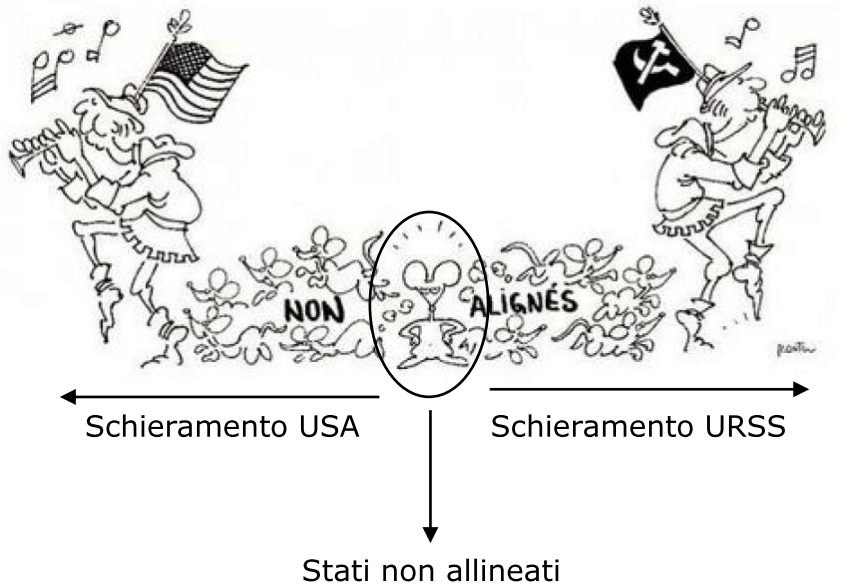
\includegraphics[width=.6\textwidth]{media/bipolarismo.png}
}

La politica di contenimento degli Stati Uniti era mirata a limitare l'espansione sovietica,
intervenendo soprattutto in Asia, America Latina e Medio Oriente.

La tensione tra i due blocchi si manifestava attraverso alleanze militari e aiuti economici,
esercitando un'influenza politica e militare in zone strategiche a livello globale.

\hypertarget{brettonwoods}{\subsubsection{Accordi di Bretton Woods}}
Gli accordi di Bretton Woods ridefinirono l'economia globale dopo la Seconda guerra mondiale.\\
Nel 1944, giudati da Stati Uniti e Gran Bretagna, le principali potenze vittoriose scelsero di
abbandonare il protezionismo\footnote{politica economica che limita le importazioni mediante
dazi e restrizioni per proteggere le industrie nazionali.} a favore di un sistema di commercio
espanso e regole economiche internazionali, per prevenire crisi finanziarie simili a quella del
1929. \vspace*{1.5cm}
\pagebreak

Il valore delle monete fu ancorato al dollaro americano, garantito in oro, permettendo una
gestione economica controllata nei diversi paesi. Questa decisione portò alla creazione di
tre istituzioni fondamentali:
\begin{itemize}
    \item Fondo Monetario Internazionale (FMI);
    \item Banca Internazionale per la Ricostruzione e lo Sviluppo (BIRS);
    \item Accordo generale sulle tariffe doganali e sul commercio (GATT), predecessore
        dell'Organizzazione Mondiale del Commercio (WTO).
\end{itemize}

Queste istituzioni promossero la stabilità monetaria, il finanziamento per la ricostruzione e
lo sviluppo e il commercio multilaterale. I risultati furono significativi:
quasi tre decenni di crescita economica continua, periodo conosciuto come 
\underline{``Età dell'oro del capitalismo regolamentato"}.

\paragraph{Accordi di Bretton Woods: Riassunto} \phantom{}

Gli accordi erano basati sulle conseguenze della crisi del 1929 ed erano mirati ad evitare che
nascessero tensioni post-sanzioni belliche globali. Gli obiettivi principali erano:
\begin{itemize}
    \item Espandere il commercio internazionale;
    \item Accordare regole vincolanti per le espansioni del commercio;
    \item Adeguare i cambi delle valute con un sistema stabile.
\end{itemize}

Le dirette conseguenze agli accordi di Bretton Woods furono la nascita dei seguenti corpi economici:
\begin{itemize}
    \item Fondo Monetario Internazionale (FMI);
    \item Banca Internazionale per la Ricostruzione e lo Sviluppo (BIRS);
    \item Accordo generale sulle tariffe doganali e sul commercio (GATT, diventato WTO nel 1995)
\end{itemize}

\subsubsection{I ``Trenta gloriosi"}
Il termine ``Trenta gloriosi'' si riferisce al periodo di notevole crescita economica in Europa
dal 1950 al 1973.

Quest'era è caratterizzata dalla ricostruzione post-bellica, dall'espansione dell'economia di
mercato e dall'intervento dello Stato sociale, portando a una ridistribuzione più equa della
ricchetta e a una significativa riduzione della disoccupazione. 

Le sue principali caratteristiche furono:
\begin{itemize}
    \item Stato sociale estero (Welfare State):\\ Stato che si impegna a garantire il benessere dei cittadini,
    investendo significamente in salute pubblica e altri servizi sociali;
    \item Aumento dei posti di lavoro $\Longleftrightarrow$ Diminuzione della disoccupazione;

    \item Forte crescita economica.
\end{itemize}

Le ragioni e le cause del boom economico furono:
\begin{itemize}
    \item Stabilità del nuovo sistema economico;
    \item Nuovi accordi sul commercio mondiali (\hyperlink{brettonwoods}{\color{blue}\underline{Bretton Woods}});
    \item \hyperlink{marshall}{\color{blue}\underline{Piano Marshall}};
    \item Progressi nella ricerca scientifica ed evoluzione tecnologica;
    \item Boom di natalità demografica;
    \item Imposizione e diffusione del modello Fordista:\\
        Assegnazione di singole parti di produzione di un grande progetto composto da molteplici parti;
    \item Disponibilità di fonti energetiche a basso prezzo (petrolio e gas naturale).
\end{itemize}

\pagebreak

\subsection{L'eta della Crisi (1973 - 1991)}
\subsubsection{Modello socialdemocratico}
Il modello socialdemocratico rappresenta un approccio politico ed economico che fonde aspetti
del capitalismo con un robusto intervento dello Stato, mirato a garantire il benessere sociale.
Questo modello si basa su uno Stato sociale (Welfare State).

Le sue principali caratteristiche sono:
\begin{itemize}
    \item Sostegno attivo delle istituzioni europeiste e internazionali (es. ONU);
    \item Integrazione dei sindacati e organizzazioni dei lavoratori nei processi decisionali
        economici e sociali, favorendo la negoziazione collettiva per migliorare le condizioni
        lavorative;
    \item Diritti civili, libertà individuale e partecipazione democratica che garantisce un
        sistema politico aperto e inclusvo;
    \item Economia di mercato equilibrata tra un settore privato dinamico e un aiuto significativo
        dello Stato.\\ L'equità fra sistema statale e privato è chiamato Statalismo.
\end{itemize}

\subsubsection{Crisi petrolifera del 1973}
Le più grandi crisi del petrolio si verificarono nel 1973 e nel 1979.

Il settore delle compagnie petrolifere nel dopoguerra venne influenzato da svariati fattori
politici: gli Stati Uniti decisero di tagliare la produzione petrolifera per dare priorità
alla conservazione delle risorse.\\
Questa decisione portò a un importante incremento di produzione nel Medio Oriente, Africa
Settentrionale e Unione Sovietica.

Come prima conseguenza, nel 1973 l'\underline{OPEC (Organizzazione dei Paesi Esportatori di Petrolio)}
incrementò i prezzi del petrolio. 

L'inflazione e la scarsità petrolifera influenzò la sua fornitura mondiale e portò allo
sviluppo di nuovi metodi di approvvigionamento energetico e allo studio di nuovi metodi per
generare energia a basse emissioni.

Le conseguenze della crisi petrolifera furono:
\begin{itemize}
    \item Coscienza di una necessità del risparmio energetico:
    \begin{itemize}
        \item Sviluppo di nuove tecnologie;
        \item Studio per un'efficienza energetica maggiore;
    \end{itemize}
    \item Dipendenza dal petrolio ridotta;
    \item Potenziamento di fonti energetiche alternative (carbone, gas naturale, nucleare, ...);
    \item Sostituzione di materiali ad alto costo energetico (alluminio, acciaio) con materiali
        più ecosostenibili (plastiche, leghe);
    \item Incentivi per il riciclaggio e per le attività a basso consumo energetico.
\end{itemize}

\subsubsection{L'ondata liberista in occidente}
\paragraph*{Fine del modello socialdemocratico (ca. 1975)} \phantom{}

Gli anni '70 furono segnati dalle crisi petrolifere che causarono inflazione e stagnazione
economica (stagflazione) nei paesi occidentali. Ciò mise in difficoltà i governi
socialdemocratici che faticavano a mantenere il Welfare State senza aumentare il debito pubblico.

Il modello socialdemocratico fu criticato per la sua inefficienza economica e la pesante
burocrazia. Parallelamente nacque una corrente di pensiero che promuoveva il mercato libero e
la riduzione del ruolo dello Stato nell'economia.

\paragraph*{Crisi del Sistema Comunista} \phantom{}

Molti paesi comunisti soffrivano di bassa produttività, scarsa qualità dei beni, innovazione
limitata e inefficiente ripartizione delle risorse.

Leader come Gorbačëv tentarono di riformare il sistema sovietico con politiche come la 
Perestrojka e la Glasnost, ma queste riforme non riuscirono a prevenire il collasso politico.

Il sistema comunista in Europa orientale crollò tra la fine degli anni '80 e l'inizio degli
anni '90, iniziando con la cadutoa del Muro di Berlino nel 1989 e terminando con la fine
della Guerra fredda e la dissoluzione dell'Unione Sovietica nel 1991.

\paragraph*{Ondata liberista} \phantom{}

La fine degli anni '70 e '80 videro l'ascesa di leader che promisero politiche di
deregolamentazione, privatizzazione e tagli fiscali.

L'ondata liberista coincise con un'accelerata globalizzazione, che favorì la libera circolazione
di capitali, beni e servizi a livello globale, aumentando la competizione e l'efficienza 
economica.

Sebbene l'ondata liberista abbia portato a significativi tassi di crescita economica in molti 
paesi, fu criticata per aver aumentato la disuguaglianza di reddito e per aver ridotto la rete
di sicurezza sociale, specialmente nei paesi precedentemente socialdemocratici.
\pagebreak

\section{La globalizzazione tra XX e XXI secolo}
\subsection{La geografia del comportamento}
Dal documento: \href{https://github.com/matteofrongillo/passerella/blob/main/Geografia/media/Pass_03a_GlobalizzazioneXX-XXI-A_22-23.pdf?raw=true}{La geografia del comportamento}

\subsubsection{Globalizzazione e cambiamenti geopolitici}
Dopo la Seconda Guerra Mondiale, il mondo è passato da un equilibrio bipolare durante la Guerra
fredda alla supremazia unipolare degli Stati Uniti seguendo il crollo dell'URSS.

Questo cambio ha facilitato accordi economici transcontinentali come il NAFTA (North American Free Trade Agreemen)
e l'espansione dell'APEC (Gruppo di cooperazione economica Asia-Pacifico), che hanno promosso la
liberalizzazione del commercio e incrementato la cooperazione economica tra i continenti.

\subsubsection{Impatti sociali ed economici}
Nei decenni '80 e '90, l'indebitamento crescente nei paesi in via di sviluppo, aggravato da
politiche monetarie restrittive come quelle degli Stati Uniti, ha portato a profonde crisi
economiche.

Le condizionalità imposte dal FMI (Fondo Monetario Internazionale), come le riforme strutturali
e le politiche di austerità, hanno spesso esacerbato le difficoltà economiche nei paesi in via
di sviluppo, peggiorando la miseria e l'instabilità sociale.

\subsubsection{Evoluzione tecnologica e impatto economico}
L'epoca post-bellica fino gli anni '70 è stata dominata dal modello fordista-keynesiano, che ha
favorito una produzione di massa basata su economie di scala. Questo modello è stato
gradualmente sostituito dal toyotismo e dalla produzione snella, le quali hanno introdotto una
maggiore flessibilità ed efficienza nella produzione.

La seconda metà del XX secolo ha visto un forte impulso verso la finanziarizzazione 
dell'economia, con la rivoluzione informatica che ha trasformato le economie globali, facilitando
una maggiore transnazionalizzazione e diminuendo il controllo statale.

\begin{figure}[h!]
    \centering
    \begin{tabular}{|l|l|}
        \hline 
        \textbf{Fordismo} & \textbf{Post-fordismo} \\
        \hline 
        \begin{tabular}{@{}l@{}}
            - Modello di organizzazione industriale \\ 
            \; tipico nel Novecento
        \end{tabular} & 
            - Modello organizzativo post-industriale \\
        \hline 
        \begin{tabular}{@{}l@{}}
            - Predominantemente nel Settentrione \\
            \; europeo e in America nel dopoguerra
        \end{tabular} & 
        \begin{tabular}{@{}l@{}}
            - Emergenza a partire dagli anni '70 e ' 80 \\
            \; del Novecento
        \end{tabular} \\
        \hline 
        \begin{tabular}{@{}l@{}}
            - Produzione in serie di grandi \\
            \; stabilimenti
        \end{tabular} & 
            - Flessibilità produttiva \\
        \hline 
        \begin{tabular}{@{}l@{}}
            - Produzione basata sulla \\
            \; standardizzazione e sull'efficienza
        \end{tabular} & 
        \begin{tabular}{@{}l@{}}
            - Produzione differenziata, mirata alla \\
            \; personalizzazione
        \end{tabular} \\
        \hline 
        \begin{tabular}{@{}l@{}}
            - Economia basata sull'espansione di \\
            \; mercati potenzialmente infiniti
        \end{tabular} & 
        \begin{tabular}{@{}l@{}}
            - Produzione di piccoli lotti, spesso in \\
            \; base alla domanda
        \end{tabular} \\
        \hline 
        \begin{tabular}{@{}l@{}}
            - Uso intensivo della forza lavoro \\
            \; umana
        \end{tabular} & 
        \begin{tabular}{@{}l@{}}
            - Maggiore uso di tecnologie e \\
            \; automatismi
        \end{tabular} \\
        \hline 
        \begin{tabular}{@{}l@{}}
            - Stabilimenti come quelli della Ford \\
            \; negli Stati Uniti
        \end{tabular} & 
        \begin{tabular}{@{}l@{}}
            - Decentrare la produzione spostandola \\
            \; vicino ai mercati target
        \end{tabular} \\
        \hline 
        \begin{tabular}{@{}l@{}}
            - Innovazione focalizzata su processi e \\
            \; tecnologia che ottimizzano la \\
            \; produzione in serie \\
            - Vertice del modello con le grandi
        \end{tabular} & 
        \begin{tabular}{@{}l@{}}
            - Innovazione orientata alla \\
            \; diversificazione e all'adattamento rapido \\
            - Emergenza di nuovi poli produttivi \\
            \; flessibili e decentrati
        \end{tabular} \\
        \hline 
        & 
        \begin{tabular}{@{}l@{}}
            - Maggiore interconnessione con \\
            \; l'economia globale e con le reti di \\
            \; informazione \\
            - Importanza crescente delle società \\
            \; transnazionali e delle multinazionali
        \end{tabular} \\
        \hline
        \begin{tabular}{@{}l@{}}
            - Catena di montaggio (prod. in serie)
        \end{tabular} & 
            - Flessibilità, just-in-time \\
        \hline 
        \begin{tabular}{@{}l@{}}
            - Domanda in funzione all'offerta
        \end{tabular} & 
            - Offerta in funzione della domanda \\
        \hline 
        \begin{tabular}{@{}l@{}}
            - Territorializzazione
        \end{tabular} & 
            - Delocalizzazione \\
        \hline 
        \begin{tabular}{@{}l@{}}
            - Mercati specifici ``nazionali'', seppur \\
            \; comunicanti
        \end{tabular} & 
        \begin{tabular}{@{}l@{}}
            - Mercati ``transnazionali'' \\
            \; (Stati come ostacolo)
        \end{tabular} \\
        \hline
    \end{tabular}
\end{figure}

\subsubsection{Rivoluzioni digitali}
Gli anni '80 hanno visto una saturazione nei mercati di beni di consumo durevoli nei paesi
sviluppati e una riduzione nella domanda di materie prime tradizionali a favore di nuovi
materiali tecnologici.

Il cambio di secolo ha portato con sé una seconda rivoluzione digitale e una crisi delle
politiche neoliberiste, segnando una nuova era di
``\underline{capitalismo della sorveglianza e informazionale}", con significative implicazioni per
la privacy, la sicurezza e il cambiamento nei rapporti di potere globale, con una tensione
crescente tra Stati Uniti e Cina.

\subsubsection{Riassunto grafico: La geografia del comportamento}
\figbox{
    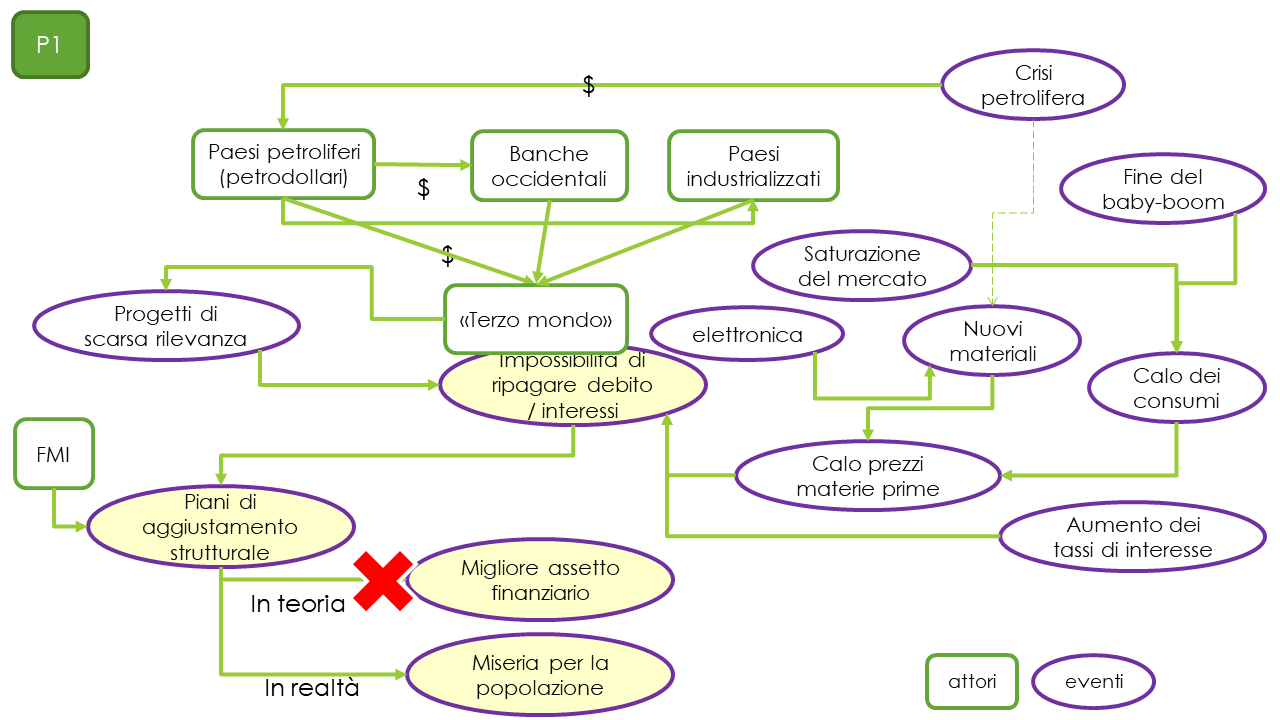
\includegraphics[width=0.95\textwidth]{media/SchemaP1.png}
}
\pagebreak

\subsection{Nuovi attori e nuove visioni per la scena internazionale }
Dal documento: \href{https://github.com/matteofrongillo/passerella/blob/main/Geografia/media/Pass_03b_GlobalizzazioneXX-XXI-B_22-23.pdf?raw=true}{Nuovi attori e nuove visioni per la scena internazionale}

\subsubsection{Ascesa della Cina come superpotenza}
L'apertura diplomatica tra Stati Uniti e Cina, nel 1973, fu vista come una mossa che permise
alla Cina di emergere come una superpotenza economica e politca, in grado di sfidare la
supremazia americana e partecipare attivamente alla globalizzazione sotto l'egida degli Stati
Uniti.

\subsubsection{Paesi di nuova industrializzazione (NIC)}
Durante la fine degli anni '80 e l'inizio degli anni '90, alcuni paesi in Asia sudorientale,
Africa australe e America Latina trasformarono le loro economie per adattarsi e partecipare ai
grandi circuiti finanziari e commerciali globali.

Accanto a questi paesi emergenti, vi furono paesi gravemente indebitati e paesi poveri con
un'industrializzazione precaria e specializzati in poche materie prime. Queste nazioni
riscontrarono difficoltà crescenti nel contesto globalizzato, evidenziando disparità nella
distribuzione dei benefici della globalizzazione.

\subsubsection{Trasizione dei paesi socialisti}
Sempre nel periodo '80-'90, i paesi socialisti, compresi l'Unione Sovietica e gli stati
dell'Europa centrale, lottarono per adattarsi al nuovo contesto economico globalizzato.
Questo portò al crollo dell'URSS e alla dissoluzione del blocco socialista.

Contrariamente ad altri paesi, la Cina mantenne il suo modello socialista, ma si aprì con
prudenza alla globalizazione, cercando di integrarsi senza rinunciare al controllo statale.

L'integrazione di nuovi attori economici e la trasformazione dei paesi socialisti
ristrutturarono significamente il panorama geopolitico globale.

\subsection{La società polindustriale}
Dal documento: \href{https://github.com/matteofrongillo/passerella/blob/main/Geografia/media/Pass_03b_Sabbatucci_Adreatta_Morin_Aime.pdf?raw=true}{La società polindustriale}

\subsubsection{Testo A: Alla ricerca dell'ordine mondiale - \textit{Andreatta}}
Il biennio tra la caduta del Muro di Berlino e la dissoluzione dell'Unione Sovietica vide
cambiamenti politici e strategici globali di portata storica.

La speranza di un nuovo ordine internazionale più pacifico e cooperativo, fondato su una
co-dominazione USA-URSS, non si realizzò. Le liberalizzazioni nei paesi comunisti innescarono
il crollo dell'URSS.

La fine dell'URSS lasciò un vuoto politico e ideologico significativo, che non fu adeguatamente
colmato dalla Russia postcomunista, portando all'emergere di nuovi nazionalismi e movimenti
politici.

\subsubsection{Testo B: I due principali scenari per il futuro formulati negli anni Novanta - \textit{Morin}}
La dissoluzione dell'equilibrio bipolare facilitò la manifestazione di conflitti localizzati e
l'ascesa di nuove sfide globali, tra cui le divisioni economiche tra Nord ricco e Sud povero, e
le tensioni culturali tra l'Occidente e il mondo islamico.

In un mondo privo di un ordine internazionale chiaro, mancò una leadership globale efficace,
rendendo il panorama internazionale più incerto e trasformando il sistema internazionale in un
terreno di conflitto e transizione inquietante.

\subsubsection{Testo C: Scontri e incontri di culture - \textit{Aime}}
Il contesto storico post Guerra Fredda mise in evidenza come i rapidi cambiamenti avvenuti alla
fine del XX secolo avessero plasmato le dinamiche internazionali, conducendo a una fase di
incertezza e transizione globale.

La crisi di leadership globale evidenziò l'assenza di una direzione chiara, con la Russia
incapace di sostituire l'URSS e gli Stati Uniti e altre potenze emergenti incapaci di gestire da
soli l'ordine mondiale.

\subsubsection{Testo A, B, C in breve}
Nel biennio 1989 (caduta del Muro di Berlino) e il 1991 (dissoluzione dell'URSS), gli
equilibri politici e strategici del pianeta subirono uno sconvolgimento di portata
paragonabile a quelli delle due Guerre mondiali.

Molti speravano che la fine della Guerra fredda portasse un nuovo ordine internazionale più
pacifico e liberale, basato su una co-dominazione tra USA e URSS. Tuttavia, le liberalizzazioni
nei paesi comunisti contribuirono al crollo dell'Unione Sovietica.

La scomparsa dell'URSS creò un vuoto politico e ideologico significativo che la Russia
postcomunista non fu in grado di colmare. Questo portò all'appirizione di nazionalismi e
tendenze politiche precedentemente sopite.

L'assenza di un equilibrio bipolare vide aumentare il numero di conflitti locali e della
creazione di contrapposizioni globali, come la suddivisione tra Nord ricco e Sud povero o
le tensioni culturali tra l'Occidente e il mondo islamico.

In un mondo privo di ordine internazionale venne a mancare una leadership globale efficace,
entrando così in una fase di transizione inqueta senza un ordine internazionale chiaramente
delineato. L'assenza di una leadership rese il panorama mondiale incerto.
\vspace*{.5cm}

\begin{center}
    \begin{tikzpicture}[
        level 2/.style = {sibling distance = 5cm}
    ]
    \node {\Ovalbox{Equilibrio conflitturale}}
        child {
            node {\ovalbox{
                    \begin{minipage}{.10\textwidth}
                        \centering Biennio '89 - '91
                    \end{minipage}
                    }
                }
            child {
                node {\ovalbox{
                        \begin{minipage}{.215\textwidth}
                            \centering Speranza:\\ 
                            Co-dominio tra USA-URSS più pacifico
                        \end{minipage}
                    }
                }
            }
            child {
                node {\ovalbox{
                        \begin{minipage}{.18\textwidth}
                            \centering Realtà:\\ 
                            Dissoluzione URSS
                        \end{minipage}
                    }
                }
                child {
                    node {\ovalbox{
                        \begin{minipage}{.27\textwidth}
                            \centering Conflitti locali, disequilibrio\\
                            e contrapposizioni globali
                        \end{minipage}
                        }
                    }
                }
            }
        };
    \end{tikzpicture}
\end{center}
\phantom{}

\subsubsection{Approfondimento sulla società polindustriale}

\paragraph{La fine della storia - \textit{Fukuyama}}
\begin{quote}
    Fukuyama vede la storia come un processo di continua 
    modernizzazione e sviluppo con un senso ben preciso. L’uomo 
    tenderebbe perciò alla forma di civiltà più elevata, e ciò trova 
    conferma nella destinazione perseguita dai flussi migratori: paesi 
    più ricchi e più sicuri. Questi ultimi, non casualmente, sono tutti 
    caratterizzati da un modello politico democratico, il che porta 
    l’autore a sostenere che l’uomo voglia aderirvi quasi per natura e 
    che, non disponendo di un’evoluzione ulteriore, la storia sia quindi 
    giunta al capolinea. -- (\textit{4F 2019-20, Gruppo 5})
\end{quote} \phantom{}

In altre parole:

Il modello caratterizzato dalla democrazia e dal libero mercato, che alla fine della Guerra
fredda si era imposto, poteva venire considerato il “punto di arrivo” di questo processo.

La tesi è stata elaborata all’inizio degli anni ’90 e che da allora gli avvenimenti hanno in
parte sconfessato o relativizzato quella visione, come l’autore spiega nell’intervista. 

\paragraph{Lo scontro delle civiltà - \textit{Huntington}} \phantom{}

Nel libro di Huntington Lo scontro delle civiltà si delinea una visione del mondo decisamente
originale che si pone in netto contrasto soprattutto con La fine della storia e l'ultimo uomo
di Francis Fukuyama. Se infatti nell'opera di Fukuyama veniva tratteggiata una vera e propria 
``fine della storia'' con l'avvento della globalizzazione guidata dalle liberaldemocrazie 
occidentali, secondo Huntington, al contrario, la fine della guerra fredda, non solo non avrebbe
portato all'affermarsi di un modello unico, ma anzi avrebbe liberato le diverse civiltà dal
giogo del bipolarismo politico ed ideologico U.S.A. - U.R.S.S., lasciandole ben più libere di
svilupparsi autonomamente con modi e tempi differenti tra loro.

Tale situazione, secondo Huntington, non sarebbe tuttavia caratterizzata da una pacifica
convivenza […]. L'osservazione di Huntington è quindi proprio che ``gli equilibri di potere tra
le diverse civiltà stanno mutando'' mentre l'``influenza relativa dell'occidente è in calo''.
Le diverse civiltà […] stanno infatti riorientandosi sia su basi ideologiche (ed è questo il
caso del comunismo di mercato che caratterizza quella Sinica) sia, soprattutto, su basi 
religiose (come succede per quella Islamica). L'idea stessa di una civiltà che si afferma sulle
altre come universale è […] del tutto sbagliata e frutto di una visione del mondo schematica e 
ancora legata ai meccanismi della Guerra fredda.

\subsection{BRIC(S)}
Dal documento: \href{https://github.com/matteofrongillo/passerella/blob/main/Geografia/media/Internazionale-BRICS-entrambi.pdf?raw=true}
{Addio ai Bric (2015) / Il vertice dei paesi emergenti in Brasile non fa scalpore (2019)}

\subsubsection{Chi sono i BRIC(S)}
I BRICS, ossia Brasile, Russia, India, Cina e Sudafrica (aggiunto a posteriori) sono un gruppo 
di cinque grandi economie emergenti volto a promuovere la cooperazione economica e politica
tra i membri e a sfidare l'ordine economico globale dominato dall'Occidente.

La caratteristica dei paesi membri sono la loro grande estensione geografica, la loro popolosità
e la loro forte crescita economica.

Ognuno dei paesi possiede un punto di forza:
\begin{itemize}
    \item Brasile: Agricoltura;
    \item Russia: Potenza energetica;
    \item India: Formazione nel campo informatico;
    \item Cina: Beni e produzioni industriali;
    \item (Sudafrica: Aggiunto per convenzione)
\end{itemize}

\subsubsection{I loro aspetti problematici}
I principali aspetti problematici dei BRICS sono:
\begin{itemize}
    \item Sviluppo eterogeneo: la Cina ha il ruolo dominante nella crescita economica;
    \item Mancanza di visione comune e possibili tensioni interne dovute alle diversità
        politiche ed economiche dei paesi membri.
\end{itemize}

\subsubsection{Addio ai BRIC - \textit{G. Dyer}}
Nel 2015, questo termine sembrava star perdendo rilevanza come blocco emergente,
poiché i paesi membri mostravano segni di divergenza economica e politica, allontanandosi
dall'idea di un fronte unito oppositore al G7.

In particolare, Brasile e Russia affrontavano gravi sfide economiche e politiche interne che
minacciavano il loro status di economie emergenti, influenzando l'interesse e l'entusiasmo verso
il gruppo.

\subsubsection{Il vertice dei paesi emergenti in Brasile non fa scalpore - \textit{P. Haski}}
Nonostante le sfide, il gruppo dei BRICS continuava a tenere vertici e a tentare di coordinare
politiche economiche tra i suoi membri, dimostrando una certa relisienza.

I BRICS cercavano di sviluppare iniziative, come la Nuova Banca di Sviluppo, la quale mirava
a finanziare progetti di sviluppo nei paesi membri e in altre economie emergenti.

Nonostante le difficoltà interne e le differenze tra i membri, il gruppo poteva ancora aspirare
a svolgere un ruolo significativo nel ridisegnare l'ordine economico globale, sfidando
l'influenza occidentale e promuovendo un'agenda più multipolare.
\pagebreak

\subsubsection{I BRICS si prendono il Global South - \textit{F. Fasulo}}
Dal documento: \href{https://github.com/matteofrongillo/passerella/blob/main/Geografia/media/ISPI_I BRICS si prendono il Global South.pdf?raw=true}{I BRICS si prendono il Global South}

Durante il quindicesimo vertice dei BRICS, è stata presa la decisione di includere sei
nuovi membri (Argentina, Arabia Saudita, Egitto, Emirati Arabi Uniti, Etiopia e Iran) a partire
dal 2024, segnando il primo significativo allargamento dal 2010. Questo movimento strategico
riflette un desiderio di rafforzare la coalizione in risposta agli eventi geopolitici globali,
come la guerra in Ucraina.

La tensione geopolitica derivante dalla guerra in Ucraina ha spinto Russia e Cina a cercare un
maggiore sostegno internazionale, mentre altre nazioni emergenti vedono l'occasione per
aumentare la loro influenza.

La Nuova Banca di Sviluppo dei BRICS sottolinea l'abilità del gruppo di promuovere cooperazione
economica, fungendo da simbolo della loro capacità organizzativa.

Nonostante l'allargamento, ci sono tensioni evidenti tra i membri su come gestire il rapporto
con l'Occidente e su altre questioni politiche. L'India e il Brasile, ad esempio, sono più
cauti sull'allargamento veloce, preoccupati che potrebbe portare a disomogeneità o a una
dominanza eccessiva della Cina.

L'allargamento porta con sé tensioni interne, specialmente riguardo il controllo della Cina e
le relazioni con l'Occidente. Il futuro dei BRICS potrebbe ridefinire il loro ruolo nella
governance globale, con eventi come il G20 che serviranno da palcoscenico per promuovere
interessi del Sud Globale.
\pagebreak

\subsection{Riassunto: La Globalizzazione tra XX e XXI secolo}
\subsubsection{Schema riassuntivo}
%=== GRAFICO POLARISMO ===
\begin{tikzpicture}
    \tikzset{box style/.style={draw, thick, rectangle, rounded corners, fill=blue!10, text=blue, font=\fontsize{12}{14}\selectfont}}
    \tikzset{line style/.style={line width=2pt, color=blue}}

    \draw[line style, fill=blue!10, rounded corners] (0,0) rectangle (15,1.5);
    \draw[thick] (4.075,-0.2) -- (4.075,1.8);
    \draw[thick] (8.9,-0.2) -- (8.9,1.8);

    \node[box style, anchor=west, minimum width=3.9cm, minimum height=1.2cm] at (0.1, 0.75) {Bipolarismo};
    \node[box style, anchor=west, minimum width=4.7cm, minimum height=1.2cm] at (4.12, 0.75) {Unipolarismo};
    \node[box style, anchor=west, minimum width=5.9cm, minimum height=1.2cm] at (8.95, 0.75) {Multipolarismo};
\end{tikzpicture}

%=== GRAFICO MULTILATERALISMO ===
\begin{tikzpicture}
    \tikzset{box style/.style={draw, thick, rectangle, rounded corners, fill=red!10, text=red, font=\fontsize{12}{14}\selectfont}}
    \tikzset{line style/.style={line width=2pt, color=red}}

    \draw[line style, fill=blue!10, rounded corners] (0,0) rectangle (15,1.5);

    \node[box style, anchor=west, minimum width=12.15cm, minimum height=1.2cm] at (0.1, 0.75) {Multilateralismo};
    \node[box style, anchor=west, minimum width=1cm, minimum height=1.2cm] at (13.85, 0.75) {};
\end{tikzpicture}

%=== LINEA DEL TEMPO ===
\begin{tikzpicture}
    \draw[thick] (0,0) -- (15,0);

    \foreach \x/\text in {0/1945, 1.5/1972, 3.67/1989-91, 8.475/2001, 11.85/2016, 13.45/2020}
        \draw (\x,-0.1) -- (\x,0.1) node[above] {\text};

    \node at (1.5,-0.35) {Nixon/Mao};
    \node at (3.67,-0.35) {Fine Guerra};
    \node at (3.67,-0.75) {Fredda};
    \draw[thick] (3.67,0.6) -- (3.67,1.5);
    \node at (8.475,-0.35) {9/11};
    \node at (8.475,-0.75) {Cina \textrightarrow OMC};
    \draw[thick] (8.475,0.6) -- (8.475,1.5);
    \node at (11.85,-0.35) {Trump};
    \draw[thick] (11.85,0.6) -- (11.85,1.5);
    \node at (13.45,-0.35) {Biden};
    \draw[thick] (13.45,0.6) -- (13.45,1.5);
    \node at (15,0) [right] {Oggi};

    %=== Legenda 1945 ===
    {\color{red}
    \node at (1.15,-1.5) {$\Delta$ Bretton Woods};
    \node at (0.385,-2) {$\Delta$ ONU};
    \node at (0.325,-2.5) {$\bullet$ BM};
    \node at (0.38,-3) {$\bullet$ FMI};
    \node at (1.22,-3.5) {$\bullet$ GATT \textrightarrow WTO};
    }

    %=== Legenda 1989 ===
    {\color{blue}
    \node at (5.22,-1.5) {$\mapsto$ Iperpotenza USA};
    \node at (4.7,-2) {$\Delta$ Economico};
    \node at (4.48,-2.5) {$\Delta$ Militare};
    \node at (4.6,-3) {$\Delta$ Culturale};
    }
    
    \draw[decorate, decoration={brace, amplitude=5pt, mirror}, line width=1pt] 
    (6,-2.7) -- (6,-1.8) node [black,midway,xshift=-0.6cm] {};
    \node[align=left, anchor=west] at (6.15, -2.28) {Hard power};

    \draw[decorate, decoration={brace, amplitude=4pt, mirror}, line width=1pt] 
    (6,-3.2) -- (6,-2.8) node [black,midway,xshift=-0.6cm] {};
    \node[align=left, anchor=west] at (6.15, -3.05) {Soft power};

\end{tikzpicture}

\subsubsection{Lista degli eventi}
\begin{itemize}
    \item Il bipolarismo conclude con la fine della Guerra fredda
        \begin{itemize}[label=\textrightarrow]
            \item 1989 - 1991: Dissoluzione dell'Unione Sovietica
            \item 1991 - 2001: Unipolarismo
        \end{itemize}
    \item Multilateralismo: Insieme di Stati e Nazioni che collaborano per un obiettivo comune
        \begin{itemize}[label=\textrightarrow]
            \item 09.11.2001: Crollo delle Torri Gemelle mostra gli USA come Stato vulnerabile:\\
                Iperpotenza culturale {\color{red}{\circled{--}}}
            \item 2001: Cina entra nell'OMC\ \textrightarrow\ Stati Uniti non sono più i più forti
                economicamente:\\ Iperpotenza economica {\color{red}{\circled{--}}}
            \item 2001 - 2008: G. W. Bush potenzia l'esercito statunitense (Guerra al Terrore):\\
                Iperpotenza militare {\color{green}{\circled{+}}}
            \item 2007: Invasione dell'Iraq fa perdere molti uomini agli USA, influendo sulla soft power:\\
                Iperpotenza militare e culturale {\color{red}{\circled{--}\circled{--}}}
        \end{itemize}
\end{itemize}
\pagebreak

\section{Storia e interpretazioni del concetto di sviluppo}
\subsection{Interpretazioni teoriche del sottosviluppo}
\subsubsection{Inferiorità culturale}
La teoria dell'inferiorità culturale vedeva i popoli colonizzati o in via di colonizzazione
culturalmente inferiori. Questa disparità culturale ha portato all'idea che senza l'influenza
europea i popoli colonizzati non avrebbero potuto raggiungere la civiltà e un maggiore sviluppo
del paese autonomamente.

\subsubsection{Determinismo ambientale}
Il determinismo ambientale è un concetto che attribuisce la casua del sottosviluppo culturale
dei popoli colonizzati a cause naturali, quali il clima caldo, i suoli aridi e la scarsità
delle risorse, implicando che l'ambiente modelli inevitabilmente il progresso sociale ed
economico dei paesi.

\subsubsection{Confutazione del determinismo ambientale}
Le evidenze suggeriscono che le condizioni naturali avverse non siano uniche dei paesi poveri:\\
Paesi prosperi come la Svizzera o Israele superano le difficoltà ambientali, come le catene 
montuose o i terreni aridi, mentre altri paesi ricchi scarseggiano in risorse.

Di conseguenza, alcuni di questi paesi confutano la teoria che, nonostante i fattori naturali
influenzino la ricchezza di uno stato, essi non predestinano al sottosviluppo.

\subsection{L'aiuto e la cooperazione allo sviluppo}
\subsubsection{Il discorso inaugurale di Truman (1949)}
Dal documento: \href{https://github.com/matteofrongillo/passerella/blob/main/Geografia/media/011_Truman 1949 Sviluppo.pdf?raw=true}
{Estratto del discorso inaugurale del presidente Harry Truman}

Lo \textbf{sviluppo} viene visto da Truman come \underline{l'applicazione del progresso
scientifico e industriale per migliorare le} \underline{condizioni di vita}, strettamente 
collegato all'utilizzo più efficace delle risorse umane e naturali e alla prosperità e alla pace
di uno Stato.

Il \textbf{sottosviluppo} invece lo descrive in termini di povertà estrema, condizioni di vita
miserabili, economie primitive e statiche, malnutrizione e malattie. Per un Paese, il
sottosviluppo è visto come un ostacolo e una minaccia non solo per il Paese che lo sperimenta,
ma anche per quelli più prosperi.

L'approccio proposto da Truman per l'aiuto allo sviluppo fu quello di un aiuto basato sulla
condivisione delle conoscenze tecniche degli Stati Uniti con i paesi più poveri, assistendoli
nel loro sviluppo autonomo. Il piano considerava un partenariato internazionale e l'investimento
di capitali da parte degli Stati Uniti nelle regioni sottosviluppate, equilibrando le garanzie
per gli investitori e la protezione degli interessi locali.

L'aiuto allo sviluppo degli Stati Uniti era concepita come un'operazione collettiva e
cooperativa, in opposizione all'antico imperialismo, mirato a un negoziato equo e democratico
tra USA e paesi sottosviluppati che traeva vantaggi reciproci.

\subsubsection{Le ragioni del sottosviluppo secondo Truman}
\begin{itemize}
    \item Inferiorità culturale:\\
        I paesi non hanno evoluto le loro usanze e la loro cultura e questo li impedisce di
        svilupparsi ulteriormente e di integrarsi per uno sviluppo;
    \item Geodeterminismo:\\
        Le cattive condizioni naturali non contribuiscono allo sviluppo;
    \item Rostow:\\
        Mancanza di infrastrutture per la produzione e la mancanza di conoscenze;
    \item Dipendenza estera:\\
        Con l'esistenza di paesi già evoluti è difficile che una nazione sottosviluppata
        non dipenda da loro.
\end{itemize}

\subsubsection{Elementi di contesto}
\begin{itemize}
    \item Contesto post-seconda guerra mondiale, con gli USA emergenti come potenza 
        vincitrice e relativamente intatta, a differenza dell’Europa, che aveva subito danni 
        notevoli e riceveva aiuti tramite il Piano Marshall;
    \item L’inizio della Guerra Fredda, contrassegnato da tensioni ideologiche e geopolitiche 
        crescenti tra gli USA e l’URSS, che ha influito sulla politica estera statunitense e 
        sulle relazioni internazionali;
    \item La situazione dei paesi di recente indipendenza, molti dei quali erano emergenti dal 
        colonialismo e cercavano un posto nel nuovo ordine mondiale, spesso come arena 
        di influenza tra le due superpotenze.
\end{itemize}

\subsubsection{Il ruolo degli Stati Uniti nel dopoguerra}
\begin{itemize}
    \item Potenza post-bellica:\\
        Gli USA sono consolidati non solo come superpotenza militare ma anche come 
        pilastro dell’economia mondiale, emergendo meno danneggiati rispetto ad altre 
        nazioni belligeranti, in particolare quelle europee;
    \item Leadership economica:\\
        La devastazione europea apre le porte agli USA per assumere un ruolo di 
        leadership nell’economia globale, fornendo loro una possibilità di influenzare e 
        modellare le politiche economiche internazionali;
    \item Il Piano Marshall:\\
        Questo programma d’aiuti è stato un chiaro segnale dell’intenzione americana di 
        aiutare nella ricostruzione dell’Europa post-guerra, promuovendo il recupero e la 
        stabilità economica come antidoto alla possibile espansione dell’influenza sovietica;
    \item Contrasto al Comunismo:\\
        L’intervento economico americano in Europa è motivato anche da obiettivi 
        geopolitici, in particolare la volontà di arginare la diffusione del comunismo e 
        assicurare che le nazioni europee rimanessero allineate con gli ideali occidentali e 
        lontane dall’orbita sovietica.
\end{itemize}

\subsection{Il modello di sviluppo classico (Rostow)}
Il modello di Rostow propone un modello lineare di sviluppo economico in 5 fasi, dalla 
società tradizionale alla società di consuma di massa. Rostow sottolinea che la crescita
economica è il motore principale del passaggio di una società da uno stadio di sviluppo al
successivo.

\subsubsection{Le 5 fasi di sviluppo}
\begin{enumerate}
    \item Tradizionale:\\
        L'economia è basata sull'agricoltura e tecnologie primitive. La crescita è lenta e la
        struttura sociale è rigida;
    \item Precondizioni per il decollo:\\
        Inizia la transizione con innovazioni tecnologiche, infrastrutture migliorate e un sistema
        finanziario che accumula capitale. Le istituzioni politiche e sociali cambiano per
        supportare lo sviluppo;
    \item Decollo:\\
        L'economia cresce rapidamente con l'industrializzazione e l'aumento della produttività.
        La modernizzazione dell'agricoltura libera manodopera per l'industria;
    \item Maturità:\\
        L'economia è diversificata e stabile, con tecnologie avanzate ampiamente adottate.
        Migliorano i livelli di vita e l'istruzione.;
    \item Consumo di massa:\\
        L'economia raggiunge un alto livello di sviluppo con abbondanza di beni e servizi.
        La popolazione ha un alto potere d'acquisto e il settore dei servizi domina l'economia.
\end{enumerate}

\subsubsection{Critiche al modello di Rostow}
\begin{enumerate}
    \item Eurocentrico:\\
        Rostow considerava il modello di sviluppo occidentale come universale, senza tenere
        conto delle diverse realtà culturali e storiche;
    \item Assenza di differenziazione:\\
        Non riconosceva le diversità tra paesi e presupponeva che tutti seguissero lo stesso
        percorso di svilippo;
    \item Linearità:\\
        Il modello assumeva una progressione lineare senza ostacoli né deviazioni;
    \item Dipendenza dagli aiuti:\\
        Non considerava l'impatto che gli aiuti esterni potessero avere nella stimolazione o
        nell'inibizione del processo di sviluppo di una Nazione.
\end{enumerate}

\figbox{
    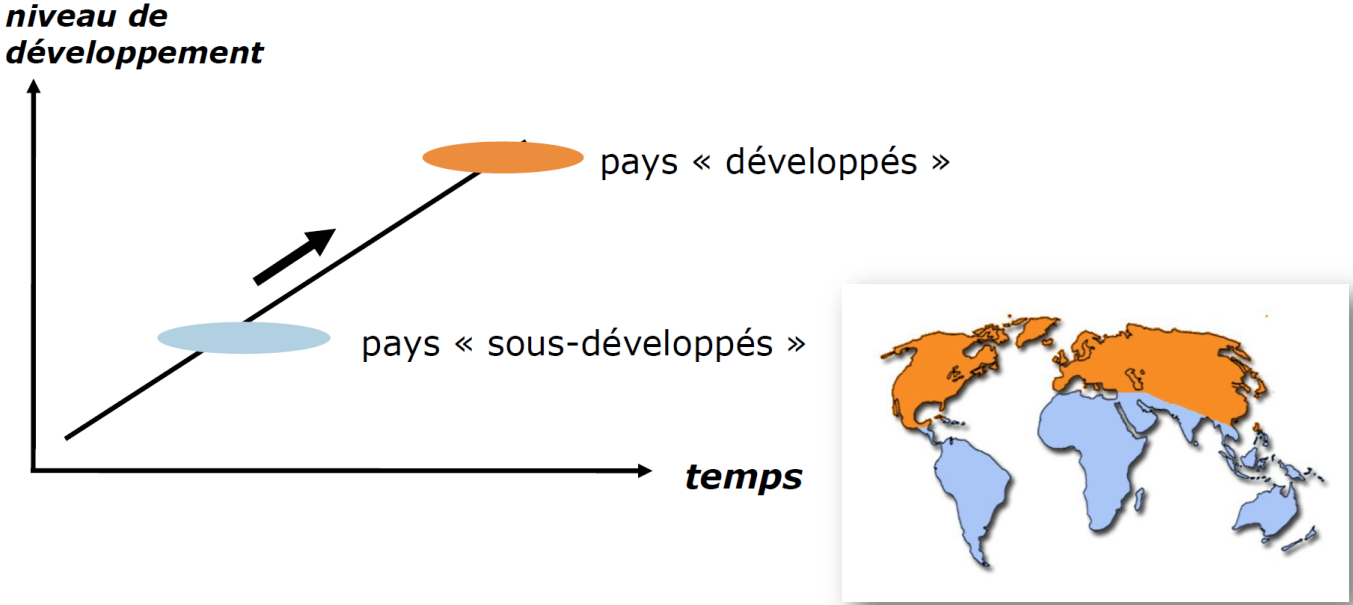
\includegraphics[width=.8\textwidth]{media/sviluppo-classico-rostow.png}
}

\subsection{La teoria della dipendenza}
La teoria della dipendenza emerge negli anni '60 e '70 come critica al modello dello sviluppo
lineare proposto da Rostow, avanzando una visione del processo di sviluppo come relazione e 
interconnessione con il commercio internazionale.

\subsubsection{Punti forti della teoria della dipendenza}
\begin{enumerate}
    \item Commercio internazionale e dipendenza:\\
        La teoria presuppone che il commercio internazionale abbia creato una divisione tra
        nazioni ``dominanti'' e nazioni ``dipendenti'', le quali dominanti controllino lo 
        sviluppo tecnologico e le risorse economiche;
    \item Cicli di indipendenza:\\
        Identificazione di un ciclo in cui le nazioni dipendenti esportano risorse e importano
        prodotti finiti, mantenendo uno stato di subordinazione economica;
    \item Imperialismo e dipendenza multinazionale:\\
        Il colonialismo e l'imperialismo vengono percepiti come le principali cause dei
        controlli multinazionali, perpetuando così la dipendenza economica;
    \item Critica alla semplificazione:\\
        La visione semplicistica delle realizioni internazionali non considera adeguatamente
        l'importanza delle politiche locali e delle dinamiche sociali nel processo di sviluppo.
\end{enumerate}

\figbox{
    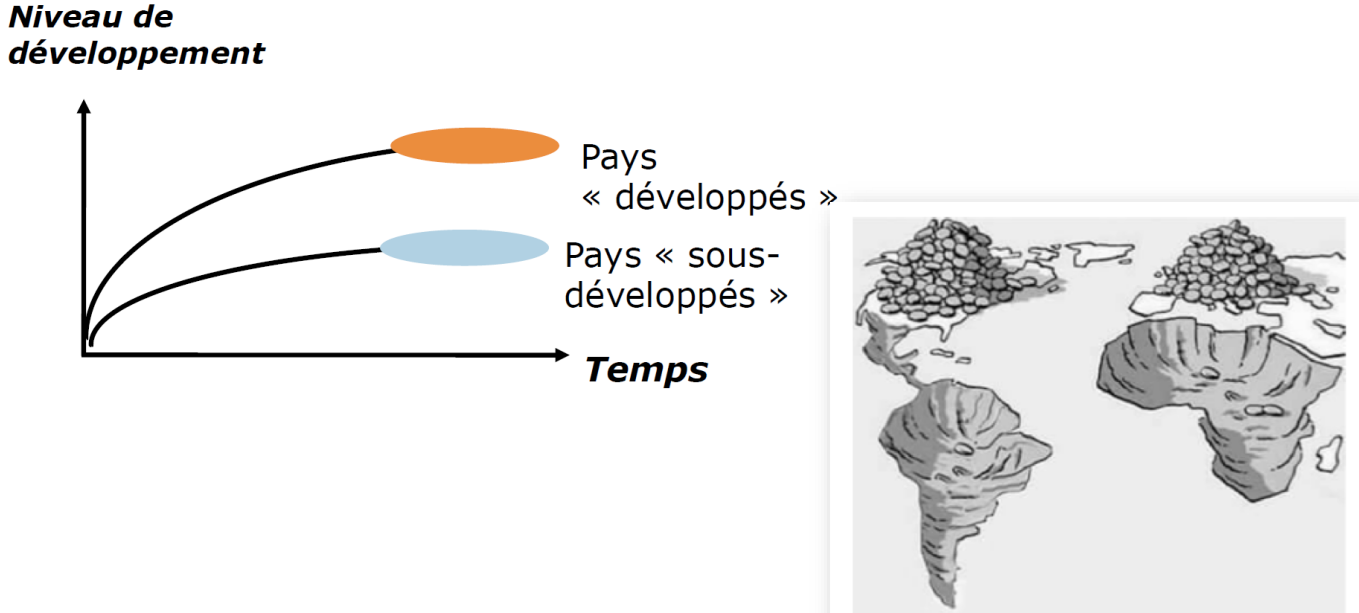
\includegraphics[width=.8\textwidth]{media/dipendenza.png}
}
\pagebreak

\subsection{Prospettive sullo sviluppo}
\subsubsection{Interpretazioni Ortodosse (sottosviluppo)}
\begin{itemize}
    \item Liberalismo:\\
        Visione lineare della storia con la convinzione che tutti i paesi seguano un percorso
        simile verso il benessere grazie al mercato e al libero scambio;
    \item Marxismo:\\
        Sviluppo visto come risultato dello sfruttamento coloniale, con un mondo diviso in
        centro (ricchi) e periferia (poveri) a causa degli scambi ineguali;
    \item Modello di Rostow:\\
        Cinque fasi di sviluppo, dal tradizionale al grande consumo di massa, con un approccio
        universalista.
\end{itemize}

\subsubsection{Interpretazioni critiche}
\begin{itemize}
    \item Ambientalismo:\\
        Sviluppo limitato dalla capacità della biosfera e dalla sostenibilità delle risorse,
        da cui derivano le nozioni ``ecosviluppo'' e ``sviluppo sostenibile'';
    \item Latouche:\\
        Sviluppo come un concetto non universalmente applicabile, che non dovrebbe seguire il
        modello occidentale e che deve essere adattato alle specificità culturali e storiche
        locali. Latouche in particolare è critico nei contronti della globalizzazione economica
        e sostiene l'idea di ``decrescita'' e sullo sviluppo basato su criteri diversi dal
        semplice aumento della produzione e dal consumo.
\end{itemize}

\subsection{Lo sviluppo sostenibile di Latouche}
\subsubsection{Serge Latouche}
Serge Latouche è un economista e filosofo francese, sostenitore del movimento della 
\textbf{decrescita}.

\subsubsection{Sviluppo e retrocessione secondo Latouche}
Secondo Latouche, la parola ``sviluppo sostenibile'' è un ossimoro, poiché una cosa che
continua all'infinito non può preservare la natura di una Terra finita.

Lo sviluppo occidentale sarebbe sostenibile se decrescesse invece di crescere, ma economicamente
non si parlerebbe di uno sviluppo ma di una \underline{retrocessione}.

\subsubsection{Il tempo della decrescita - \textit{S. Latouche}}
Dal documento: \href{https://github.com/matteofrongillo/passerella/blob/main/Geografia/media/021_Latouche Estratto 40 segg.pdf?raw=true}
{Il tempo della decrescita}
\begin{itemize}
    \item Sviluppo sostenibile come successo retorico:\\
        Lo sviluppo, che inizialmente pensato per limitare gli impatti ambientali e promuovere
        la giustizia sociale, viene criticato per non essere stato all'altezza delle
        aspettative, diventando un ``termine di moda'' più che un cambiamento effettivo;
    \item Neoliberalismo:\\
        L'ideologia neoliberalista nasce a supporto degli Accordi di Washington e le politiche
        economiche imposte ai paesi in via di sviluppo che hanno promosso il libero mercato e
        la deregolamentazione a discapito del benessere sociale e ambientale;
    \item Sviluppo occidentale e sofferenza:\\
        Critica alla tendenza del mondo occidentale a promuovere un modello di sviluppo basato
        sul proprio sistema, spesso a scapito della società e delle culture locali, causando
        disuguaglianze e sofferenze interne.
\end{itemize}

\subsubsection{Tappe nella cooperazione allo sviluppo}
\begin{enumerate}
    \item \sout{Aiuto}\ \textrightarrow\ Cooperazione allo sviluppo:\\
        Integrazione e coinvolgimento degli attori locali;
    \item Interessi propri (es. migrazioni);
    \item Cooperazione / multilateralismo per risolvere i problemi globali.
\end{enumerate}

\subsection{Indicatori e indici di sviluppo}
\subsubsection{Definizione di Indice e Indicatore}
\begin{itemize}
    \item \textbf{Indicatori:} Misurano singoli aspetti di un fenomeno (es. PIL pro capite);
    \item \textbf{Indici:} Combinano più indicatori per valutare
        complessivamente un fenomeno (es. ISU, HPI, MPI).
\end{itemize}

\subsubsection{Indici e indicatori economici}
\begin{itemize}
    \item \textbf{PIL pro capite:}\\
        Indicatore che misura il valore totale dei beni e servizi prodotti in un paese, diviso
        per la popolazione.\\
        Indica la ricchezza media per persona;
    \item \textbf{Coefficiente di Gini:}\\
        Indicatore che misura la disuguaglianza nella distribuzione del reddito all'interno di
        un paese. Valori più alti indicano maggiore disuguaglianza;
    \item \textbf{Tasso di povertà:}\\
        Indicatore che mostra la percentuale della popolazione che vive al di sotto della
        soglia di povertà estrema (meno di \$1,90 al giorno).
\end{itemize}

\subsubsection{Indici e indicatori sociali/umani e ambientali}
\begin{itemize}
    \item \textbf{Tasso di alfabetizzazione:}\\
        Indicatore che mostra la percentuale della popolazione sopra i 15 anni che sa leggere
        e scrivere. Indica il livello di istruzione;
    \item \textbf{Livello di democrazia:}\\
        Indicatore che valuta il grado di democrazia in un paese basato su vari indicatori
        di diritti politici e libertà civili;
    \item \textbf{Indice di Sviluppo Umano (ISU):}\\
    È un indice che combina PIL pro capite, tasso di alfabetizzazione e aspettativa di
    vita per valutare il benessere complessivo della popolazione;
    \item \textbf{Happy Planet Index (HPI):}\\
        Indice che misura il benessere e la sostenibilità ambientale considerando aspettativa
        di vita, soddisfazione della vita e impatto ecologico;
    \item \textbf{Indice di povertà multidimensionale (MPI):}\\
        Indice che valuta la povertà considerando vari fattori come salute, istruzione e 
        standard di vita, piuttosto che solo il reddito.
\end{itemize}
\pagebreak

\subsubsection{Human Development Report}
%=== HDR 2019-1 ===
\setlength{\intextsep}{0pt}%
\begin{wrapfigure}{l}{0.5\textwidth}
    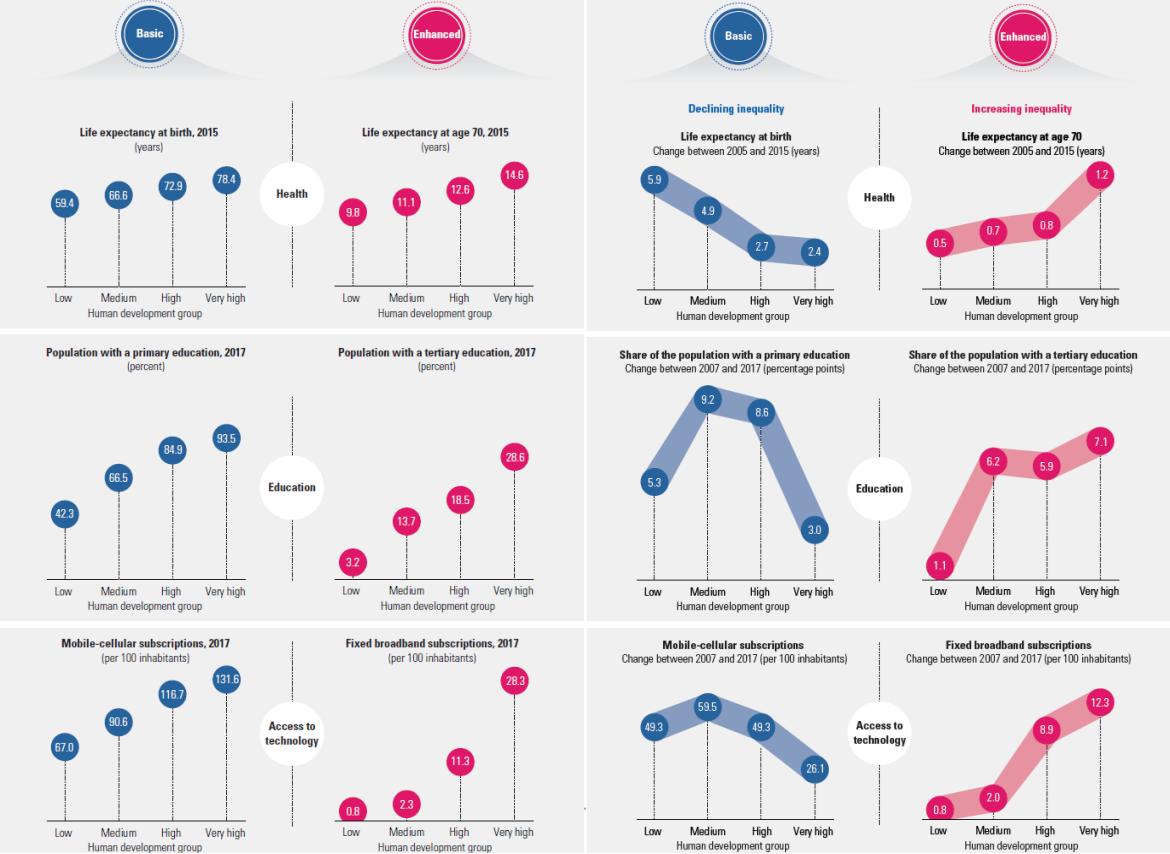
\includegraphics[width=.5\textwidth]{media/hdr2019_1.png}
    \vspace{-1cm}
\end{wrapfigure}
\textbf{HDR 2019-1}

\textbf{Titolo}: Aspettativa di vita e istruzione primaria e terziaria per gruppi di sviluppo umano,
2015-2017

\textbf{Descrizione}: Questo grafico mostra la variazione dell'aspettativa di vita alla nascita e a
70 anni, la percentuale della popolazione con istruzione primaria e terziaria, e le
sottoscrizioni mobili in base ai gruppi di sviluppo umano (basso, medio, alto, molto alto).
\wrapfill

%=== HDR 2019-2 ===
\setlength{\intextsep}{0pt}%
\begin{wrapfigure}{l}{0.5\textwidth}
    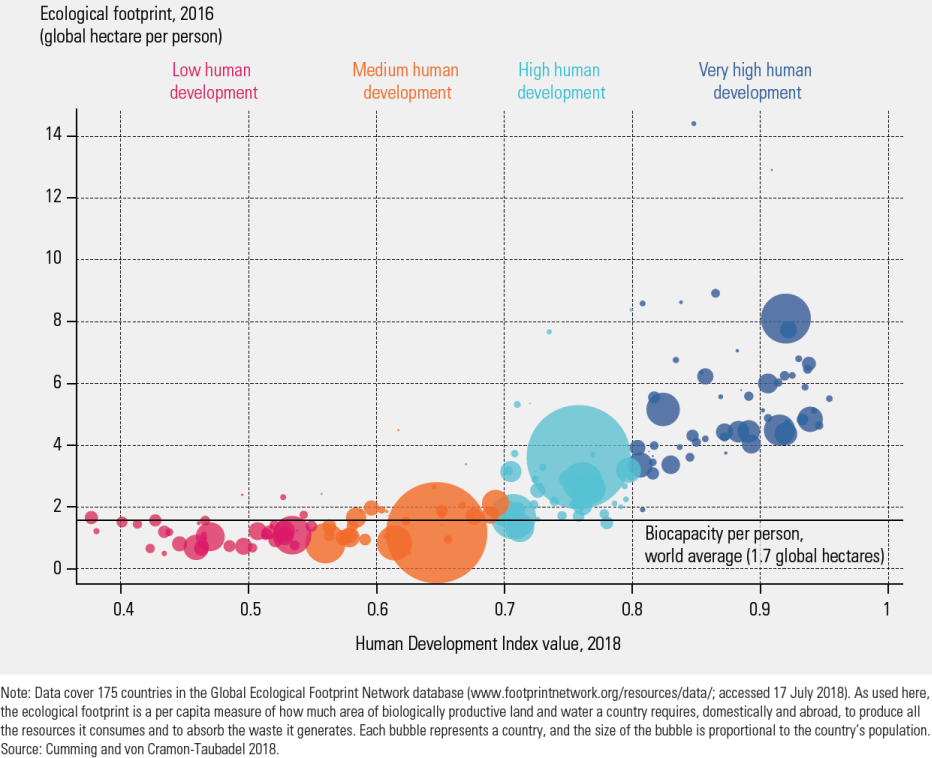
\includegraphics[width=.5\textwidth]{media/hdr2019_2.png}
    \vspace{-1cm}
\end{wrapfigure}
\textbf{HDR 2019-2}

\textbf{Titolo}: Impronta ecologica per gruppi di sviluppo umano, 2016

\textbf{Descrizione}: Questo grafico mostra l'impronta ecologica dei paesi in relazione al loro
indice di sviluppo umano, evidenziando come i paesi con alto sviluppo umano tendano ad avere
un'impronta ecologica maggiore.
\wrapfill

%=== HDR 2020-1 ===
\setlength{\intextsep}{0pt}%
\begin{wrapfigure}{l}{0.5\textwidth}
    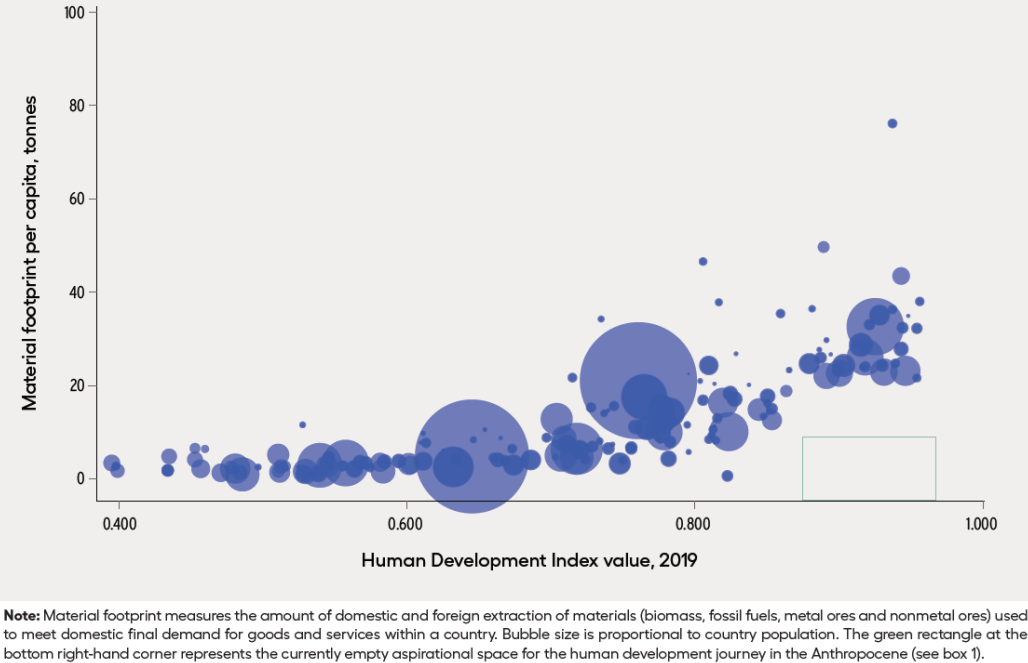
\includegraphics[width=.5\textwidth]{media/hdr2020_1.png}
    \vspace{-1cm}
\end{wrapfigure}
\textbf{HDR 2020-1}

\textbf{Titolo}: Pressione materiale e sviluppo umano, 2019

\textbf{Descrizione}: Questo grafico illustra la relazione tra l'indice di sviluppo umano e
l'impronta materiale pro capite, indicando che i paesi con un più alto sviluppo umano
esercitano una maggiore pressione materiale sul pianeta.
\wrapfill
\pagebreak

%=== HDR 2020-2 ===
\setlength{\intextsep}{0pt}%
\begin{wrapfigure}{l}{0.5\textwidth}
    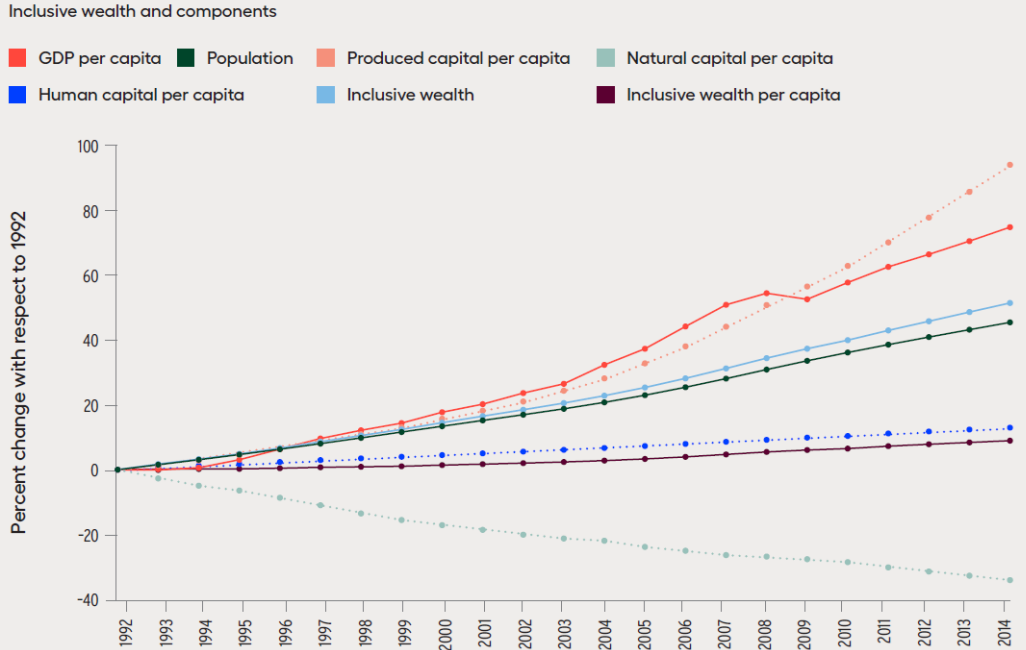
\includegraphics[width=.5\textwidth]{media/hdr2020_2.png}
    \vspace{-1cm}
\end{wrapfigure}
\textbf{HDR 2020-2}

\textbf{Titolo}: Declino del capitale naturale e aumento del PIL e del capitale umano, 1992-2014

\textbf{Descrizione}: Questo grafico mostra il declino del capitale naturale rispetto
all'aumento del PIL pro capite, della popolazione e del capitale umano, mettendo in evidenza
la perdita di risorse naturali nel tempo.
\wrapfill

%=== HDR 2020-3 ===
\setlength{\intextsep}{0pt}%
\begin{wrapfigure}{l}{0.5\textwidth}
    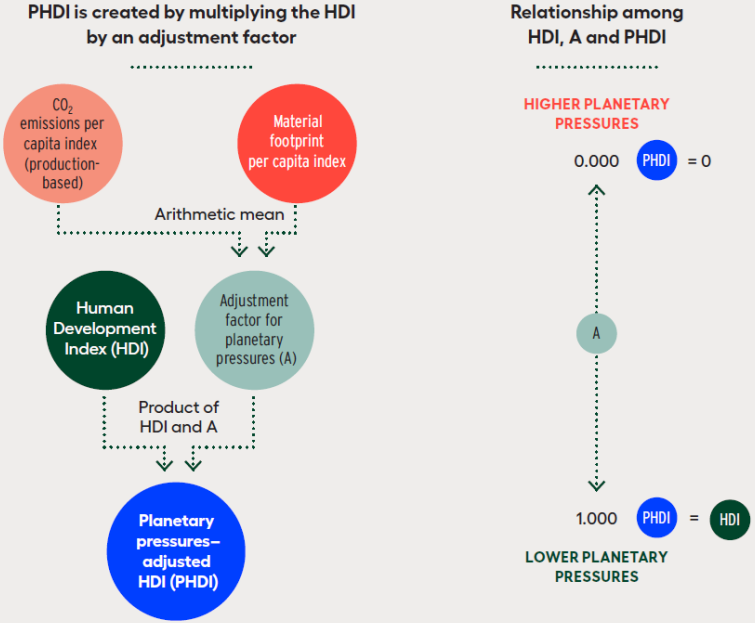
\includegraphics[width=.5\textwidth]{media/hdr2020_3.png}
    \vspace{-1cm}
\end{wrapfigure}
\textbf{HDR 2020-3}

\textbf{Titolo}: Indice di Sviluppo Umano aggiustato per le pressioni planetarie (PHDI)

\textbf{Descrizione}: Questo grafico spiega come l'indice di sviluppo umano viene aggiustato
tenendo conto delle pressioni ambientali, come le emissioni di CO2 e l'impronta materiale pro
capite, per creare il PHDI.
\wrapfill

%=== HDR 2020-4 ===
\setlength{\intextsep}{0pt}%
\begin{wrapfigure}{l}{0.5\textwidth}
    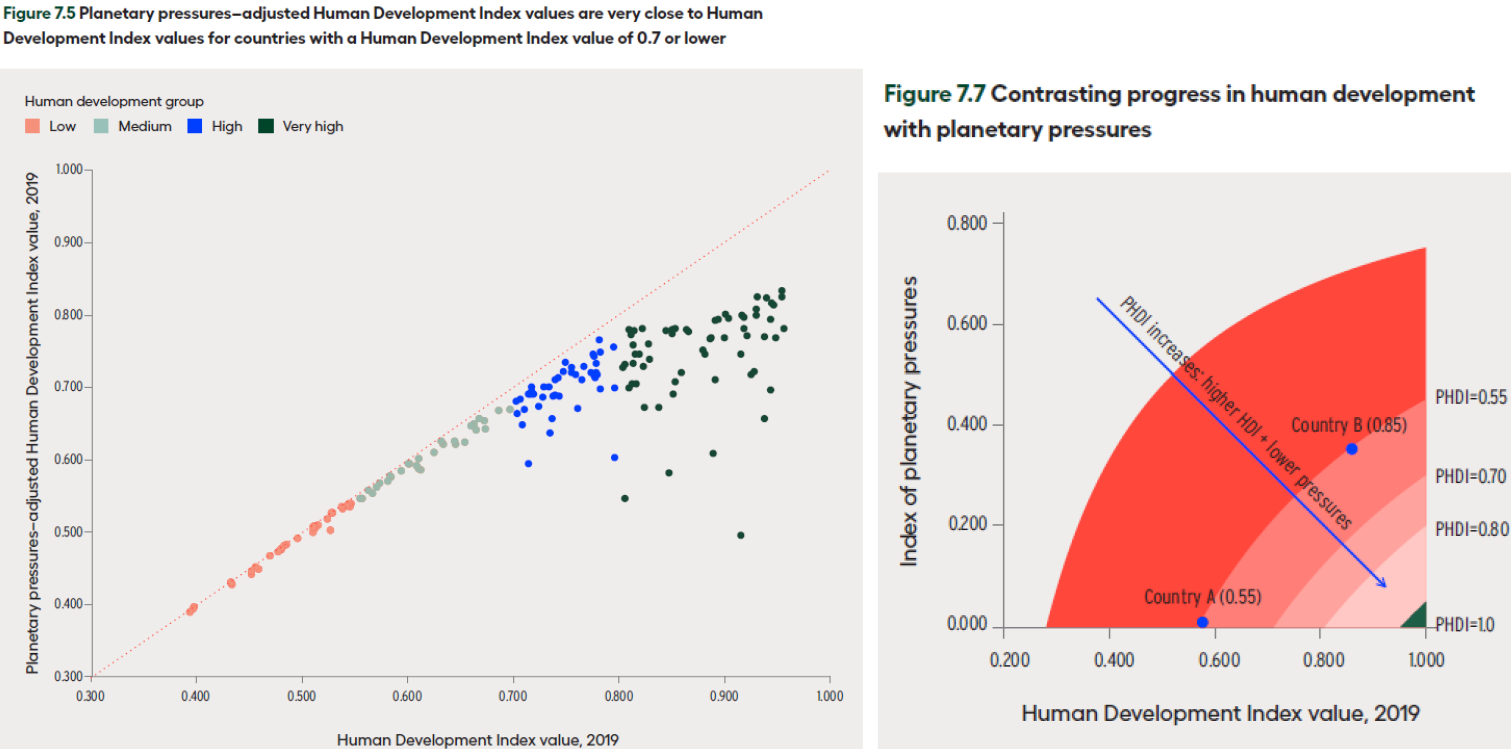
\includegraphics[width=.5\textwidth]{media/hdr2020_4.png}
    \vspace{-1cm}
\end{wrapfigure}
\textbf{HDR 2020-4}

\textbf{Titolo}: Confronto tra l'Indice di Sviluppo Umano e l'Indice di Sviluppo Umano
aggiustato per le pressioni planetarie, 2019

\textbf{Descrizione}: Questo grafico confronta i valori dell'Indice di Sviluppo Umano con
quelli aggiustati per le pressioni planetarie, evidenziando le differenze nei paesi con
diversi livelli di sviluppo.
\wrapfill

%=== HDR 2020-5 ===
\setlength{\intextsep}{0pt}%
\begin{wrapfigure}{l}{0.5\textwidth}
    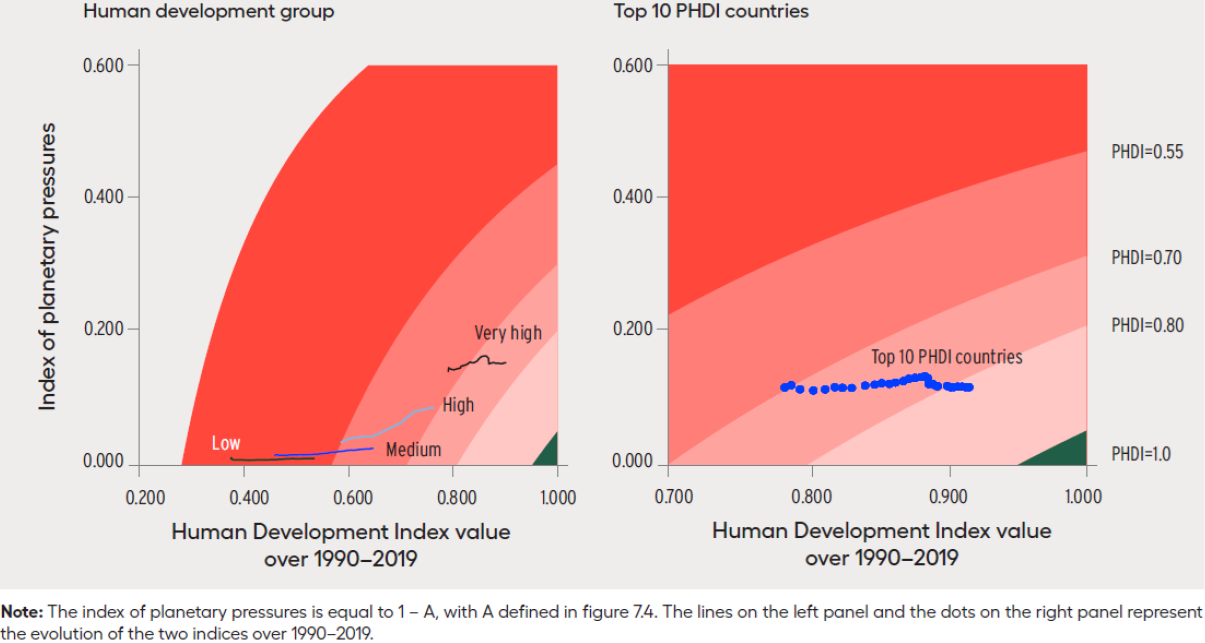
\includegraphics[width=.5\textwidth]{media/hdr2020_5.png}
    \vspace{-1cm}
\end{wrapfigure}
\textbf{HDR 2020-5}

\textbf{Titolo}: Evoluzione dell'Indice di Sviluppo Umano e delle pressioni planetarie,
1990-2019

\textbf{Descrizione}: Questo grafico mostra l'evoluzione dell'Indice di Sviluppo Umano e delle
pressioni planetarie dal 1990 al 2019, evidenziando la connessione tra lo sviluppo umano e
l'aumento delle pressioni ambientali.
\wrapfill

\subsubsection{Che cos'è lo sviluppo? - \textit{A. Greiner, G. Dematteis, C. Lanza, A. Vanolo}}
Dal documento: \href{https://github.com/matteofrongillo/passerella/blob/main/Geografia/media/031_Sviluppo-testo.pdf?raw=true}
{Geografia umana: Un approccio visuale}

\textbf{\large Fenomeno complesso:}
\begin{itemize}
    \item \textbf{Latouche:}\\
        Rappresenta una visione critia e decrescista dello sviluppo, che valorizza la diversità
        culturale e territoriale e mette in discussione i modelli dominanti occidentali.
        Latouche sostiene che lo sviluppo non debba essere misurato solo con indicatori
        economici, ma debba includere anche aspetti sociali, culturali e ambientali;
    \item \textbf{Happy Planet Index (HPI):}\\
        Questo indice valuta il benessere umano tenendo conto della sostenibilità ambientale.
        Misura l'aspettativa di vita, la soddisfazione della vita e l'impronta ecologica,
        riconoscendo così la complessità del benessere umano che non può essere ridotto solo
        a parametri economici.
\end{itemize}

\textbf{\large Semplificazione della complessità:}
\begin{itemize}
    \item \textbf{Lo sviluppo di un paese è pari alla sua crescita economica:}\\
        Questa visione riduce il concetto di sviluppo a un singolo indicatore economico,
        senza considerare altri aspetti come la distribuzione del reddito o la qualità della
        vita;
    \item \textbf{Determinare lo sviluppo di un paese tramite il PIL pro capite:}\\
        Utilizzare il PIL come unico indicatore di sviluppo è un chiaro esempio di
        semplificazione della complessità. Il PIL misura solo la produzione economica,
        ignorando aspetti umani come la salute, l'istruzione e la sostenibilità;
    \item \textbf{Stadi di sviluppo (Rostow):}\\
        La teoria di Rostow propone una sequenza di stadi universali attraverso cui tutti i
        paesi devono passare per svilupparsi. Questa visione lineare e deterministica
        semplifica la complessità delle diverse esperienze di sviluppo nei paesi poveri;
    \item \textbf{Visioni liberiste:}\\
        Le visioni liberiste promuovono il libero mercato e la crescita economica come le vie
        principali per raggiungere lo sviluppo. Tendono a ignorare le disuguaglianze sociali e
        gli impatti ambientali negativi della crescita economica;
    \item \textbf{Visioni marxiste:}\\
        Anche se opposte alle visioni liberiste, le visioni marxiste semplificano la
        complessità riducendo lo sviluppo a una questione di lotta di classe e cambiamento
        delle strutture economiche. Si concentrano principalmente sulla distribuzione della
        ricchezza e sulle dinamiche di potere economico, spesso trascurando gli aspetti 
        culturali e ambientali.
\end{itemize}
\pagebreak

\section{Demografia e flussi di persone}
\subsection{Geografia della popolazione}
\subsubsection{Preconoscenze}
\begin{itemize}
    \item Gli abitanti attuali sulla Terra sono 8.2 miliardi circa;
    \item I 5 Stati più popolati al mondo sono: Cina, India, USA, Indonesia e Pakistan;
    \item I principali Stati responsabili alla crescita della popolazione dei prossimi anni
        saranno:\\ DC Congo, Etiopia, Indonesia, Pakistan, Egitto, India, Nigeria e USA.
\end{itemize}

\subsubsection{Evoluzione della popolazione mondiali negli ultimi 50 anni}
\begin{itemize}
    \item Aumento dell'aspettativa di vita;
    \item Invecchiamento generale della popolazione\ \textrightarrow\ Fertilità $<$ Sostituzione;
    \item Maggiore assistenza sanitaria;
    \item Crescita demografica\ \textrightarrow\ Difficile da gestire.
\end{itemize}

\subsubsection{Fasi di crescita}
\begin{center}
    \begin{tikzpicture}

        \node[inner sep=0pt] (img) at (0,0) {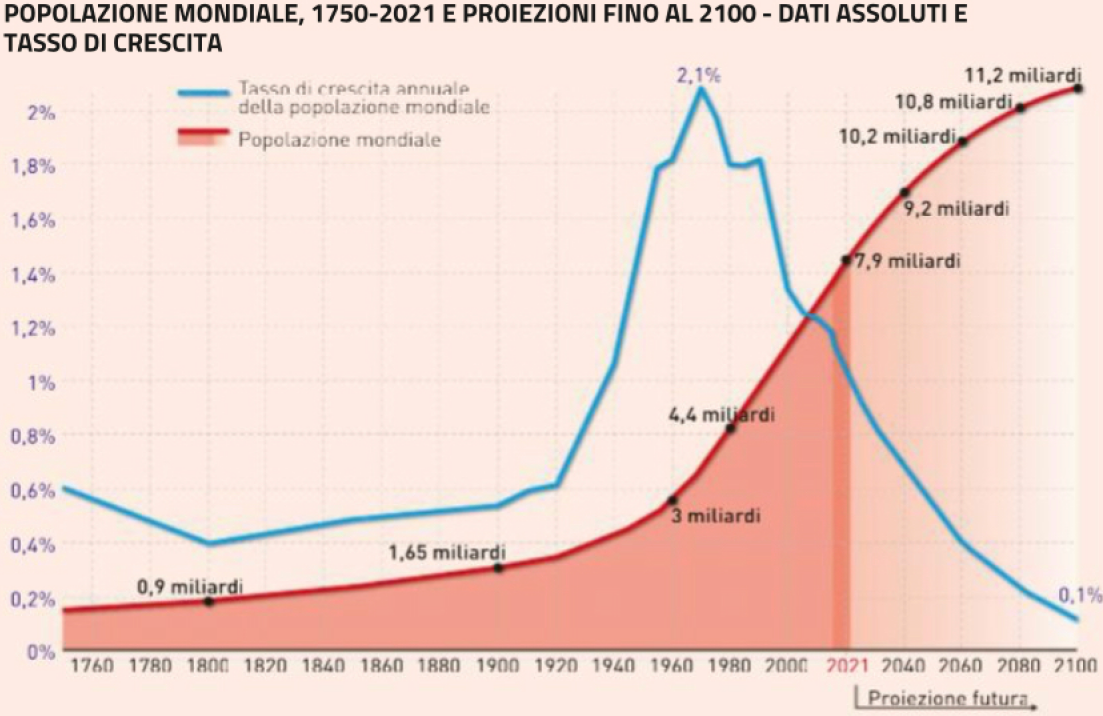
\includegraphics[width=0.8\textwidth]{media/fasi di crescita.png}};
      
        \draw[thick] (.1, -5) -- (.1, 3.5);
        \node at (-3.3,-4.8) {I$^a$ fase};

        \draw[thick] (2.37, -5) -- (2.37, 3.5);
        \node at (1.3,-4.8) {II$^a$ fase};

        \node at (4.6,-4.8) {III$^a$ fase};

    \end{tikzpicture}
\end{center}

\begin{enumerate}[label=\Roman*$^a$:]
    \item Tassi di natalità e di mortalità alti. Crescita lenta della popolazione;
    \item Calo della mortalità, ma la natalità rimane alta. Rapido aumento della popolazione;
    \item Natalità in calo, basso tasso di mortalità. Crescita demografica rallentata.
\end{enumerate}

\subsection{La distribuzione della popolazione mondiale}
\subsubsection{La distribuzione}
\begin{itemize}
    \item Il mondo rimane, come in passato, in gran parte disabitato;
    \item La distribuzione della popolazione è poco omogenea.
\end{itemize}
\pagebreak 

\subsection{Indici e modelli demografici}
\subsubsection{Concetti base}
\begin{itemize}
    \item \textbf{Tasso di natalità:} numero di nascite sul totale della popolazione (\textperthousand);
    \item \textbf{Tasso di mortalità:} numero di morti sul totale della popolazione (\textperthousand);
    \item \textbf{Tasso di crescita naturale:} differenta tra il tasso di natalità e mortalità (\textperthousand);
    \item \textbf{Saldo demografico:} somma di saldo di natalità e saldo migratorio;
    \item \textbf{Saldo naturale:} differenza tra il numero di nascite e il numero di decessi.
\end{itemize}

\subsubsection{Condizioni di fertilità}
\begin{itemize}
    \item \textbf{Aspetti che aumentano la fertilità:}
        \begin{itemize}[label=$\circ$]
            \item Maggiore manodopoera;
            \item Mortalità infantile.
        \end{itemize}
    \item \textbf{Aspetti che riducono la fertilità:}
        \begin{itemize}[label=$\circ$]
            \item Maggiore età media al matrimonio;
            \item Livelli di istruzione più elevati;
            \item Maggiore accesso all'istruzione;
            \item Costi di mantenimento dei figli più alti.
        \end{itemize}
\end{itemize}

\subsection{Il modello della tansizione demografica}
La transizione demografica è la riduzioni da tassi elevati di natalità e mortalità a tassi
con più bassi, con varie fasi intermedie di adattamento sociale ed economico.

\subsubsection{Transizione demografica nel regime tradizionale}
\begin{itemize}
    \item \textbf{Regime demografico tradizionale:}
        \begin{itemize}
            \item Alta natalità: per compensare la mortalità e per forza lavoro agricola;
            \item Alta mortalità: dovuta a malattie, carenze sanitarie e nutrizionali;
        \end{itemize}
    \item \textbf{Popolazioni del regime tradizionale:}
        \begin{itemize}
            \item Presenti in alcune zone rurali o in paesi in via di sviluppo;
            \item Accesso limitato a cure mediche e contraccettivi;
        \end{itemize}
\end{itemize}

\subsubsection{Transizione demografica nella società moderna}
\begin{itemize}
    \item \textbf{Regime demografico moderno:}
        \begin{itemize}
            \item Bassa natalità: per cambiamenti culturali, accesso ai contraccettivi, carriera;
            \item Bassa mortalità: grazie ai miglioramenti della salute e delle tecnologie mediche;
        \end{itemize}
    \item \textbf{Società del regime moderno:}
        \begin{itemize}
            \item Presente nei paesi industriali e alcuni emergenti;
            \item Elevati standard di vita, istruzione avanzata e sanità pubblica.
        \end{itemize}
\end{itemize}
\pagebreak

\subsubsection{Le 4 fasi della transizione demografica}
\phantom{}

\figbox{
    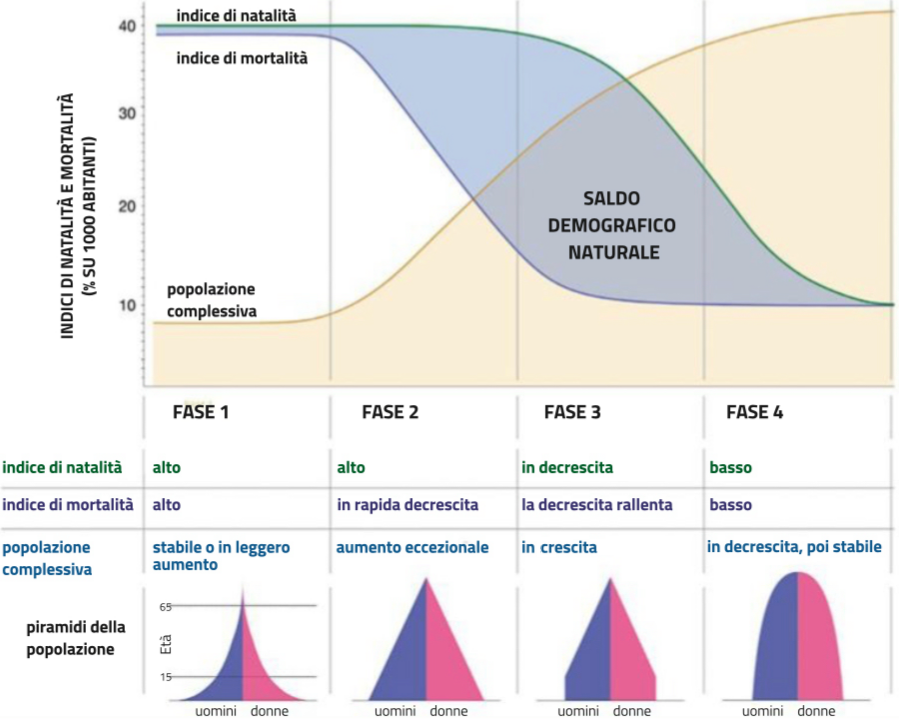
\includegraphics[width=.85\textwidth]{media/4 fasi transiozione demografica.png}
}
\phantom{}

\begin{enumerate}[label=Fase \arabic*:]
    \item Si ha un regime demografico tradizionale;
    \item La speraza di vita aumenta e la natalità aumenta;
    \item Nascono più persone di quante ne muoiano;
    \item Si arriva a un regime demografico moderno.
\end{enumerate}
\pagebreak

\subsection{Piramidi della popolazione}
\subsubsection{La struttura delle piramidi}
La struttura del grafico delle età di un Paese fornisce ulteriori informazioni sulla
popolazione di uno Stato:

\subsubsection{Le quattro forme base}

%=== PIRAMIDE A BASE ALLARGATA ===
\setlength{\intextsep}{0pt}%
\begin{wrapfigure}{r}{.4\textwidth}
    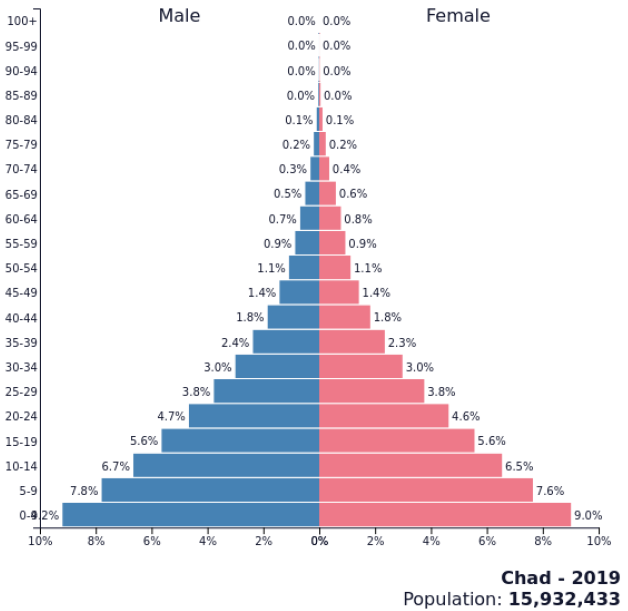
\includegraphics[width=.4\textwidth]{media/piramide a base allargata.png}
    \vspace{-1cm}
\end{wrapfigure}
\textbf{Piramide a base allargata}

\begin{itemize}
    \item Tasso di natalità alto (ev. in aumento);
    \item Tasso di mortalità omogeneo già dalle fasce più giovani;
    \item Popolazione in (leggera) crescita, alta percentuale giovani.
\end{itemize}
\wrapfill

%=== PIRAMIDE ===
\setlength{\intextsep}{0pt}%
\begin{wrapfigure}{l}{.4\textwidth}
    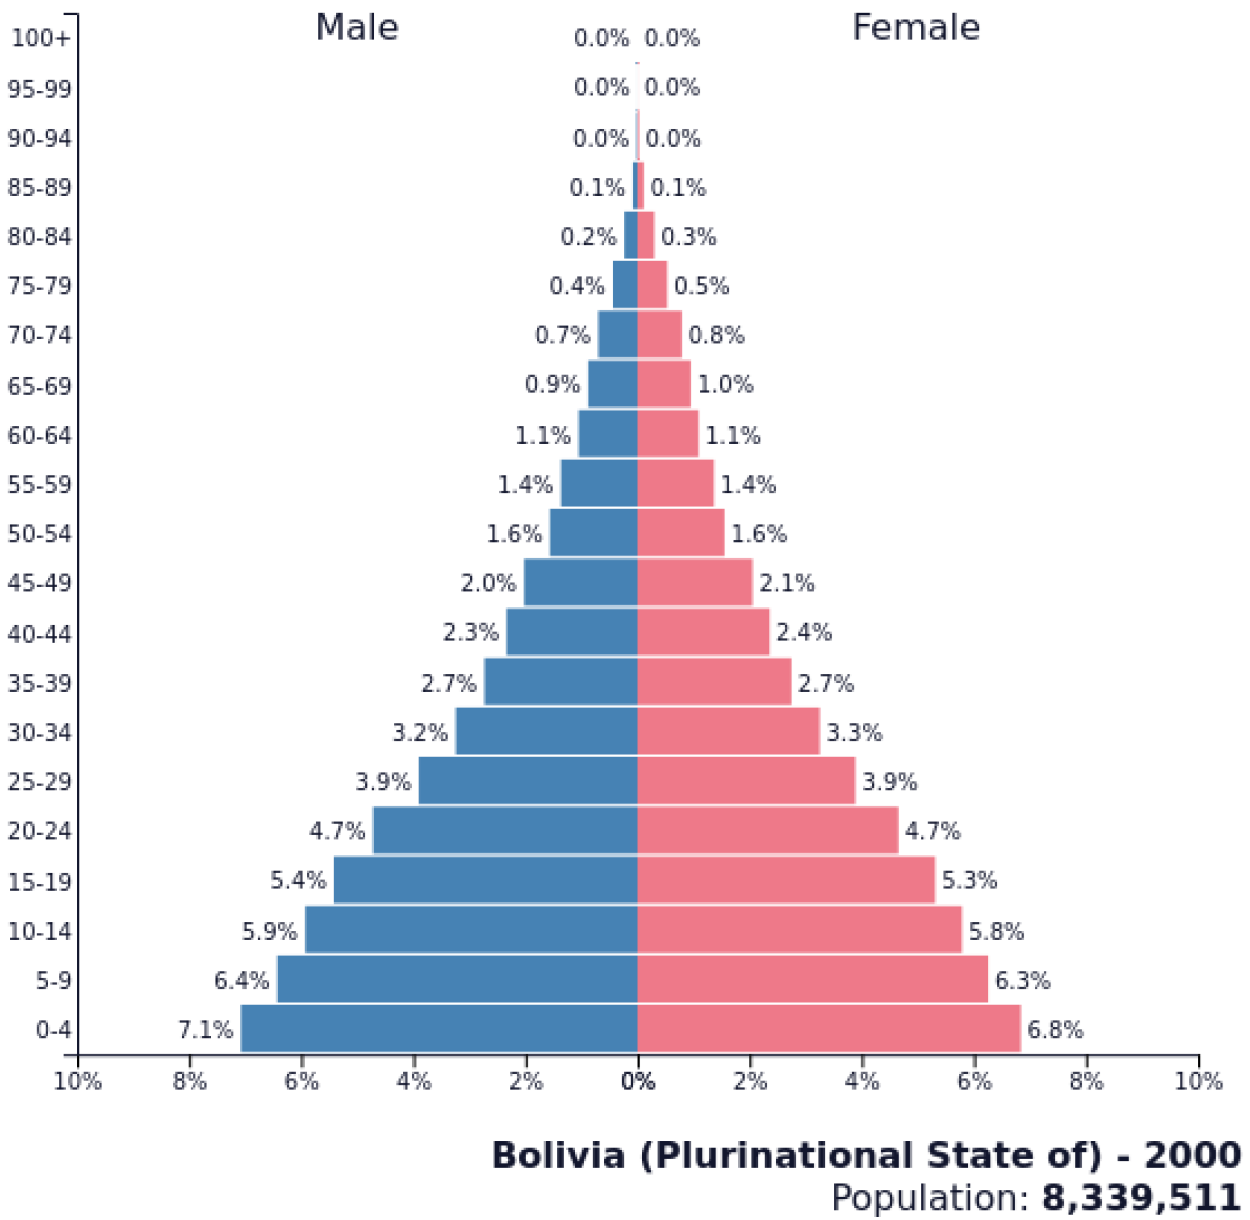
\includegraphics[width=.4\textwidth]{media/piramide demografica.png}
    \vspace{-1cm}
\end{wrapfigure}
\textbf{Piramide}

\begin{itemize}
    \item Tasso di natalità alto;
    \item Tasso di mortalità in diminuzione, distribuito omogeneamente su tutte le fasce;
    \item Popolazione in (forte) aumento.
\end{itemize}
\wrapfill

%=== CAMPANA ===
\setlength{\intextsep}{0pt}%
\begin{wrapfigure}{r}{.4\textwidth}
    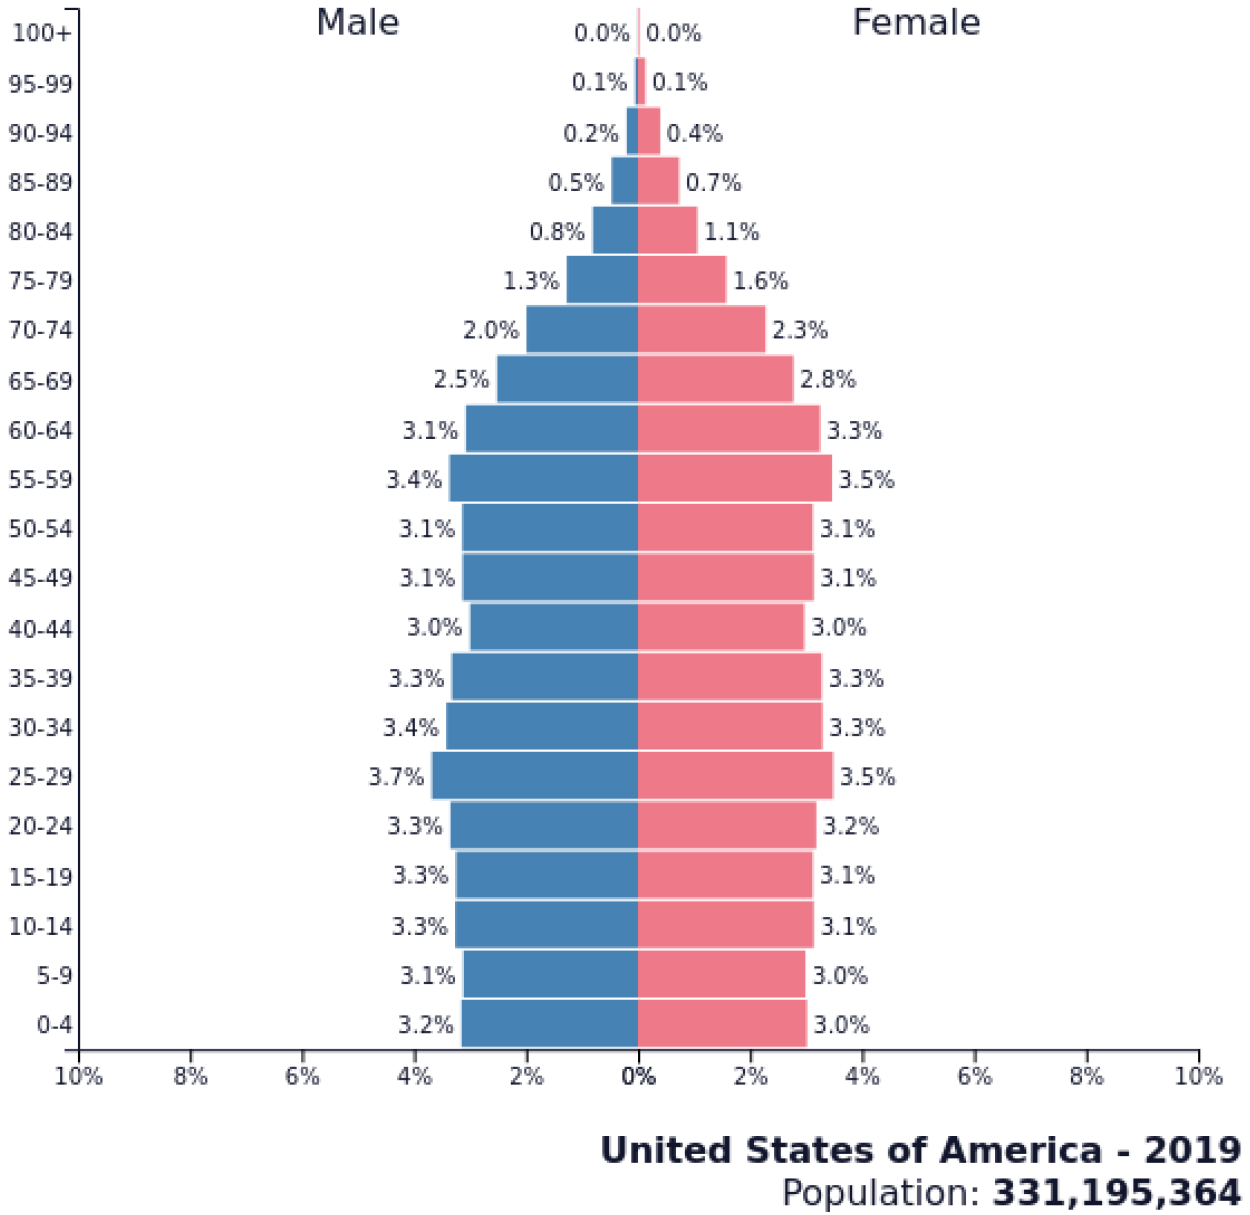
\includegraphics[width=.4\textwidth]{media/campana.png}
    \vspace{-1cm}
\end{wrapfigure}
\textbf{Campana}

\begin{itemize}
    \item Tasso di fecondità pari a circa 2.1 figli per donna;
    \item Speranza di vita alta, tassi di mortalità relativamente alti a partire dalla terza età;
    \item Popolazione stabile.
\end{itemize}
\wrapfill

%=== URNA ===
\setlength{\intextsep}{0pt}%
\begin{wrapfigure}{l}{.4\textwidth}
    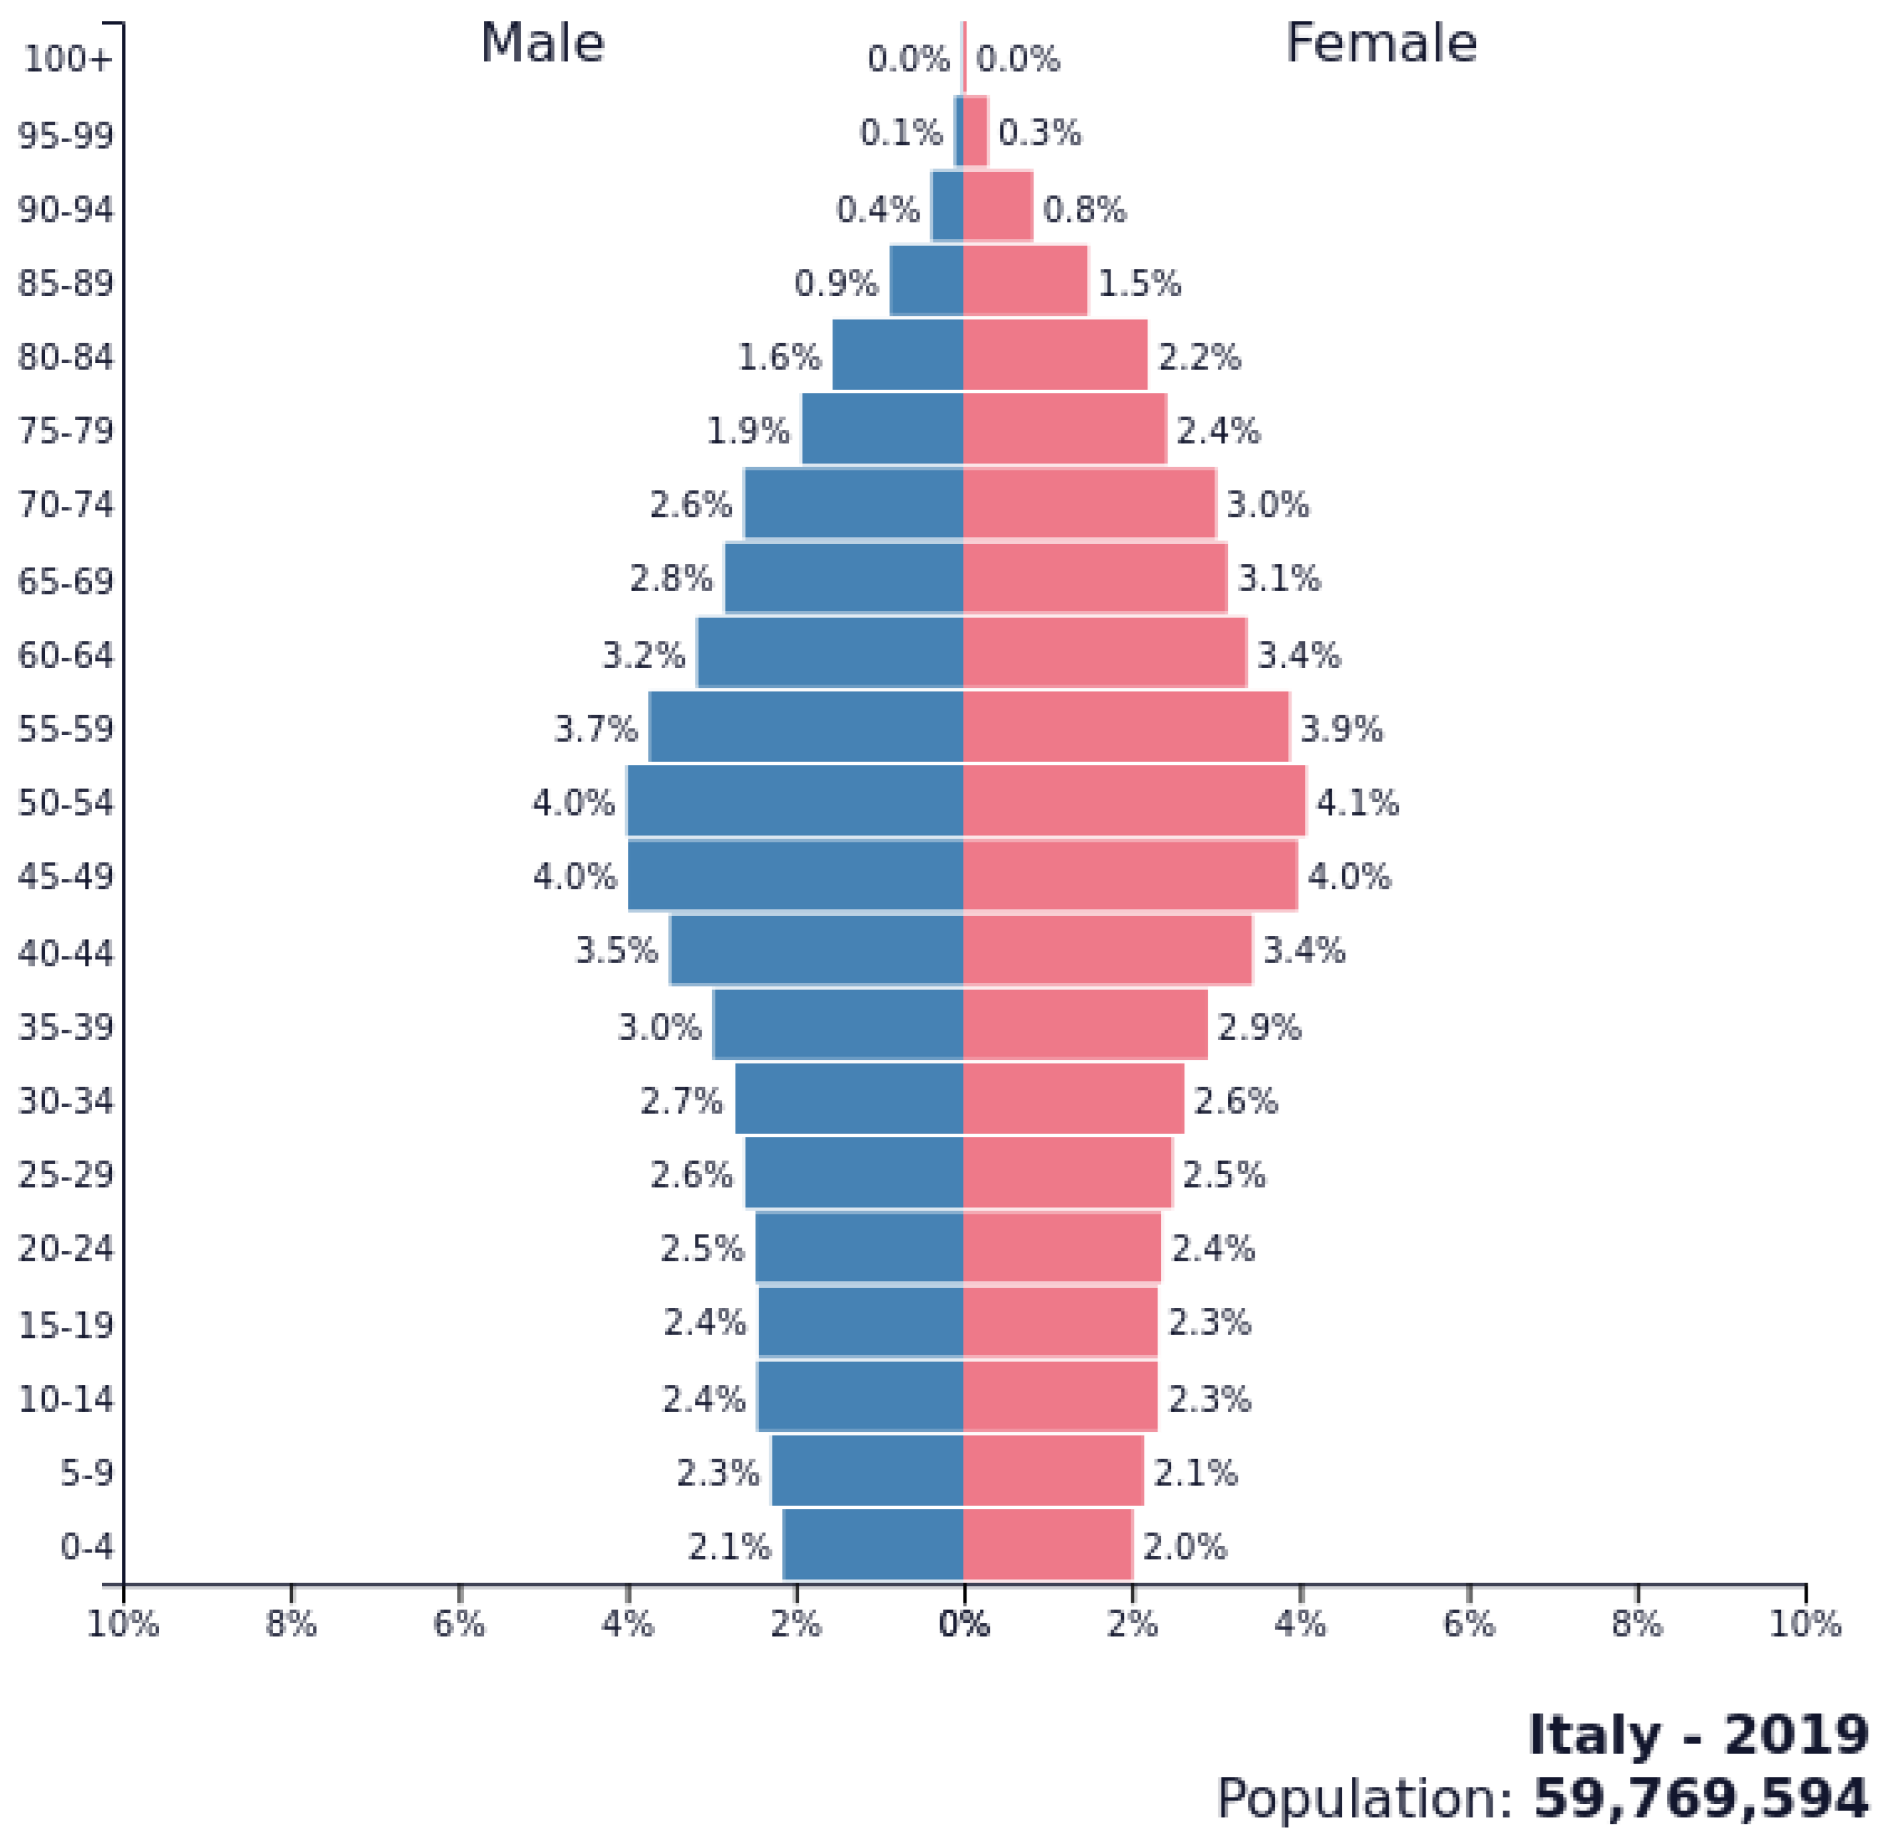
\includegraphics[width=.4\textwidth]{media/urna demografica.png}
    \vspace{-1cm}
\end{wrapfigure}
\textbf{Urna}

\begin{itemize}
    \item Tasso di fecondità bassi (meno di 2.1 figli per donna);
    \item Alta percentuale di persone anziane, speranza di vita alta, tassi di mortalità alti
        dalla terza età;
    \item Popolazione in diminuzione e in invecchiamento.
\end{itemize}
\wrapfill

\subsection{Dinamiche demografiche a livello mondiale}
\subsubsection{Eventi eccezionali}
\begin{itemize}
    \item Guerre:\\
        Comportano allo stringimento della parte bassa-centrale;
    \item Baby boom:\\
        Sostanzioso allargamento della base;
    \item Medoti contraccettivi:\\
        Propensione a una geometria ad urna.
\end{itemize}

\subsubsection{Situazioni di immigrazioni ed emigrazioni}
\begin{itemize}
    \item La crescita economica di un paese aumenta:
    \begin{itemize}[label=$\circ$]
        \item Immigra forza lavoro dall'estero;
        \item In genere gli immigranti hanno tra i 25 e i 35 anni;
        \item Spesso lasciano il Paese al termine della carriera lavorativa;
    \end{itemize}
    \item La crescita economica di un paese diminuisce:
    \begin{itemize}[label=$\circ$]
        \item La popolazione trova lavoro all'estero ed emigra;
        \item La quantità di denaro inviata al paese natio dagli emigranti corrisponde a una
            buona parte del PIL.
    \end{itemize}
\end{itemize}

\subsection{Le migrazioni internazionali}





\end{document}
